\documentclass{standalone}
\usepackage{tikz}
\usepackage{amsmath}
\usetikzlibrary{patterns,decorations.markings,backgrounds}
\usetikzlibrary{arrows.meta}

\def\a{-15}
\def\d{4}
\def\w{15}
\def\b{\w-\a}
\def\eps{0.5}
\def\wall{0.5}
\def\h{20}
\def\r{0.25}

\def\textscale{2}

% mesh points

\def\gapY{0,-0.0576162637510319,-0.1216343344151953,-0.1927655233372393,-0.2718001768620555,-0.3596164591139486,-0.4571901056129607,-0.5656052674577866,-0.6860665590585615,-0.8199124381306454,-0.9686300806960866,-1.133871906860673,-1.317473936719028,-1.52147619144181,-1.748145363476987, -2.0, -2.251854635661703,-2.47852380827835,-2.682526063474919,-2.866128093715104,-3.031369920183381,-3.18008756298665,-3.313933442240199,-3.434394733974975,-3.542809895914013,-3.640383542510802,-3.728199824759525,-3.807234478295241,-3.87836566721447,-3.942383737858097}

\def\gapX{0,0.07420761769380471,0.1662470919969679,0.2804033720488498,0.4219910554789618,0.5976018146389315,0.8154112914314402,1.085559717532598,1.420623983017105,1.836203145435822,2.351644689162638,2.990945249321639,3.783867759914917,4.76732709630521,5.987108674145053,7.500000000000000,8.584114756007992,9.519759946657405,10.32726848353328,11.02418868113149,11.62566562262247,12.1447702631542,12.5927834948759,12.9794412910326,13.31314628126745,13.60115035892204,13.84971226211021,14.06423360255622,14.24937623663608,14.40916357688694,14.54706803217206,14.66608646498921,14.76880531218977,14.85745680962387, 14.93396747834954,15}


\def\outsideGapX{-8,-6.341652079869036,-5.01497373494099,-3.953631063057665,-3.104556921181095,-2.425297599075961,-1.881890143741698,-1.447164189085495,-1.099383426161848,-0.8211588138148889,-0.5985791233905262,-0.4205153690241437,-0.2780643607306086,-0.1641035566132647,-0.07293491851229295,15.06139887086819,15.12961983187678,15.2054209019263,15.28964431828457,15.38322589444375,15.48720542124966,15.60273822792749,15.73110801493105,15.87374111105214,16.03222232858628,16.20831256894115,16.40396839160717,16.62136375296846,16.86291415516176,17.13130348758319,17.42951385554307,17.76085870867358,18.12901965657548,18.53808737419692,18.99260706202659,19.49762893830041,20.05876435390513,20.68224815083901,21.37500792800405,22.14474101615037,23}


\def\outsideGapBIGQUADSX{-14.98104603324309,-13.20938635390576,-11.4554432672083,-9.719039612037918,23.85155796640447,24.70739509578187,25.56753290726427,26.43199302530591,27.30079714315083,28.17396709819299,29.05152483620297,29.93349241223902}

\def\outsideGapBIGQUADSY{0.6089743698635424,1.50641026471989}

\begin{document}
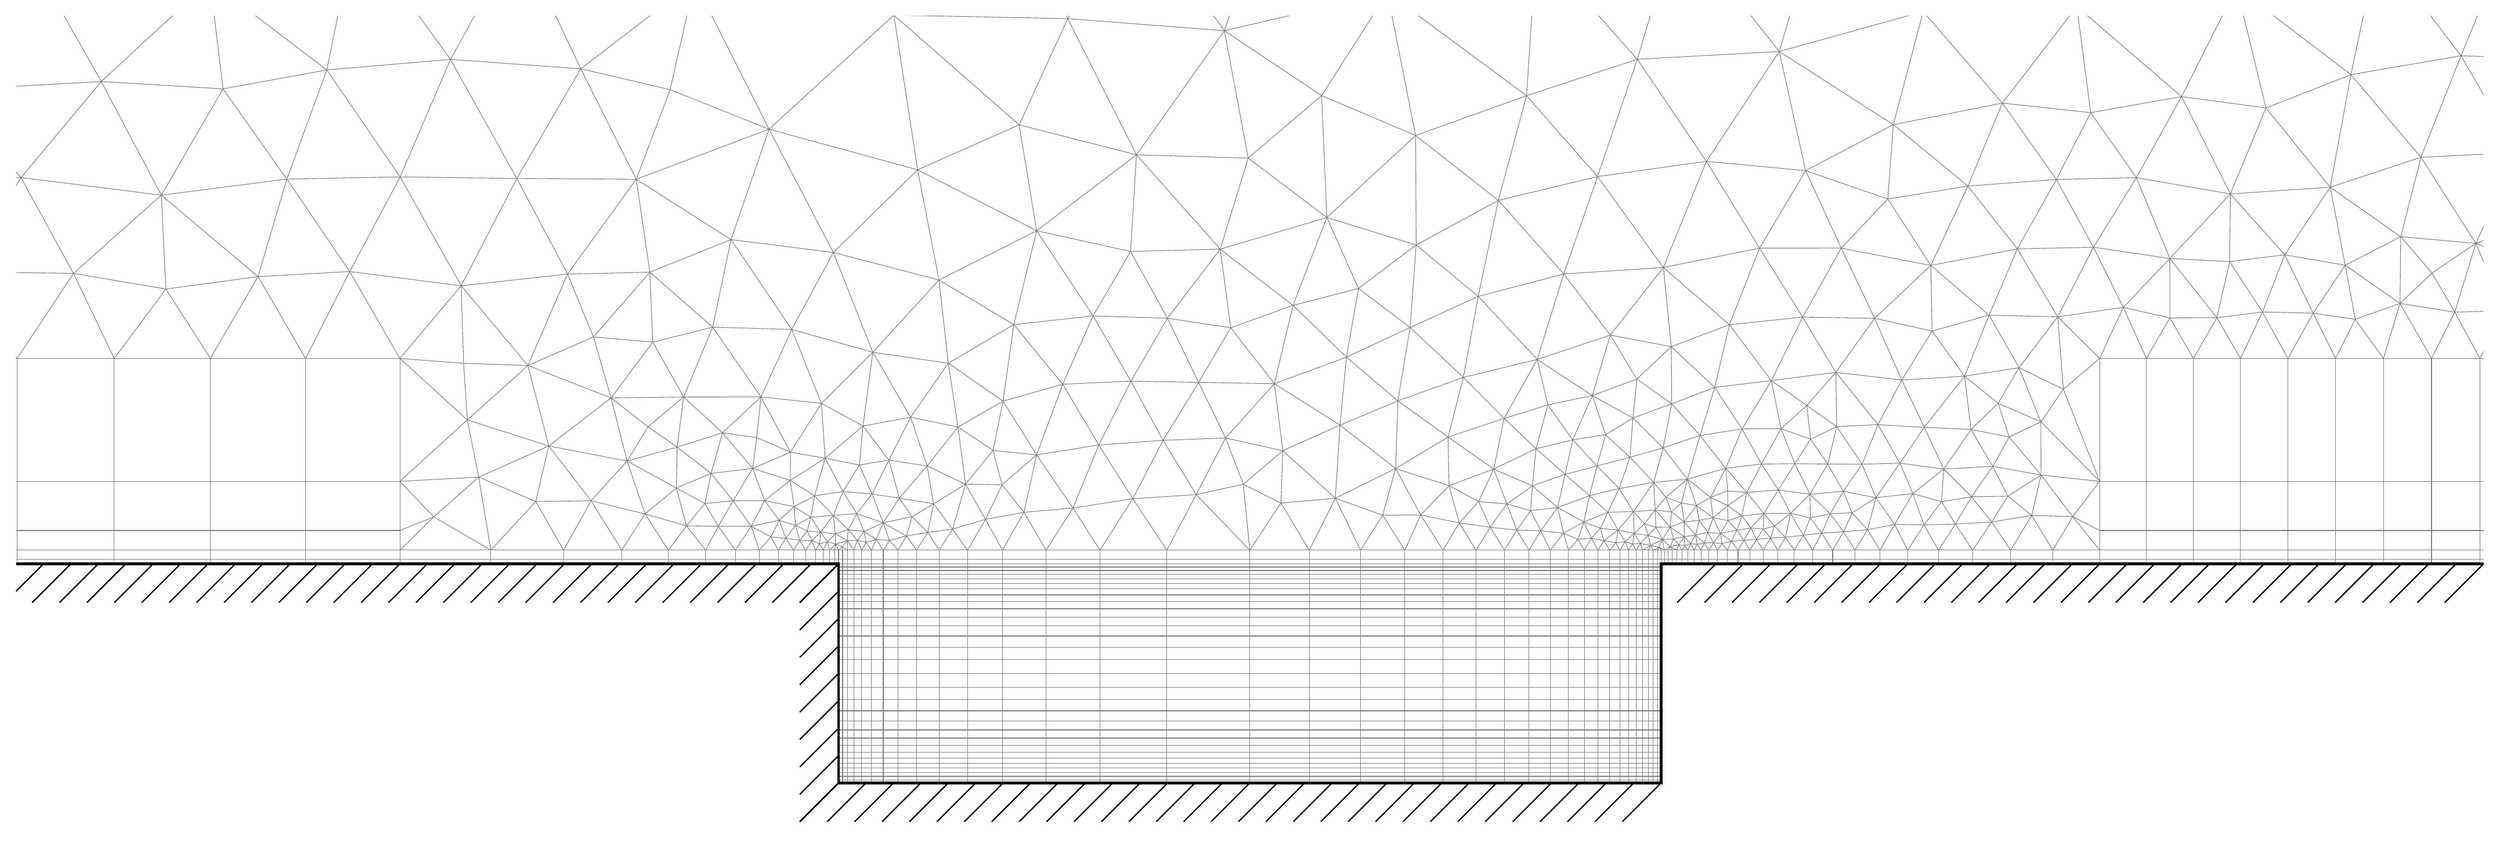
\begin{tikzpicture}[scale=1.2]
% crop tikz image
\def\xmin{-15}
\def\xmax{30}
\def\ymin{-4.8}
\def\ymax{10}
\clip (\xmin,\ymin) rectangle (\xmax,\ymax);


\def\lengthWall{1.0}
\foreach \x in {-15,-14.5,...,0,16,16.5,...,30} {
    \draw[thick] (\x,0) -- ++(225:\lengthWall); % Wall hatching
}
\foreach \x in {0,0.5,...,15} {
    \draw[thick] (\x,-\d) -- ++(225:\lengthWall); % Wall hatching
}
\foreach \y in {0,-0.5,...,-4} {
	\draw[thick] (0,\y) -- ++(225:\lengthWall); % Wall hatching
}

%%%%%%%%%%%%% quads %%%%%%%%%%%%%%%
% mesh inside gap
\foreach \y in \gapY {
    \draw[thin,gray] (0,\y) -- (\w,\y);
}
\foreach \x in \gapX {
	\draw[thin,gray] (\x,\r) -- (\x,-\d);
}
\draw[thin,gray] (\a,0.0833333) -- (\b,0.0833333);
\draw[thin,gray] (\a,0.25) -- (-8,0.25);
\draw[thin,gray] (23,0.25) -- (\b,0.25);


% mesh outside gap
\foreach \x in \outsideGapX {
	\draw[thin,gray] (\x,0) -- (\x,\r);
}
\foreach \x in \outsideGapBIGQUADSX {
	\draw[thin,gray] (\x,0) -- (\x,3.75);
}
\foreach \y in \outsideGapBIGQUADSY {
	\draw[thin,gray] (\a,\y) -- (-8,\y);
	\draw[thin,gray] (23,\y) -- (\b,\y);
}

%%%%%%%%%%%%%%%%%%%%%%%%%%%%%%%%%%%

%%%%%% triangle mesh  (done automatically with msh2tikz.py script) %%%%%%
\draw[thin,gray] (-0.05467873372482963,0.3612721642325018) -- (-0.1641035566132647,0.25);
\draw[thin,gray] (-0.05467873372482963,0.3612721642325018) -- (0.1596724319421445,0.4219466340059819);
\draw[thin,gray] (-0.05752389816359533,0.5500736575350326) -- (-0.05467873372482963,0.3612721642325018);
\draw[thin,gray] (-0.05752389816359533,0.5500736575350326) -- (-0.3277298669310191,0.578773416668771);
\draw[thin,gray] (-0.05752389816359533,0.5500736575350326) -- (0.1755033747620929,0.6251281517511262);
\draw[thin,gray] (-0.07293491851229295,0.25) -- (-0.05467873372482963,0.3612721642325018);
\draw[thin,gray] (-0.07293491851229295,0.25) -- (0.0,0.25);
\draw[thin,gray] (-0.09503169481057061,5.684587878970147) -- (-0.8538089253916414,4.278932758501862);
\draw[thin,gray] (-0.09503169481057061,5.684587878970147) -- (-1.960998843073157,5.919177237864387);
\draw[thin,gray] (-0.09503169481057061,5.684587878970147) -- (0.6253354693960566,3.862219877921509);
\draw[thin,gray] (-0.09503169481057061,5.684587878970147) -- (1.442102142299169,7.192982734660184);
\draw[thin,gray] (-0.09685870183355899,0.8841742374236521) -- (-0.05752389816359533,0.5500736575350326);
\draw[thin,gray] (-0.09685870183355899,0.8841742374236521) -- (-0.4370640500322395,1.241481991007586);
\draw[thin,gray] (-0.09685870183355899,0.8841742374236521) -- (0.08107811557776737,1.320633968173347);
\draw[thin,gray] (-0.1641035566132647,0.25) -- (-0.07293491851229295,0.25);
\draw[thin,gray] (-0.2014451644788208,0.4022397542291494) -- (-0.05467873372482963,0.3612721642325018);
\draw[thin,gray] (-0.2014451644788208,0.4022397542291494) -- (-0.05752389816359533,0.5500736575350326);
\draw[thin,gray] (-0.2014451644788208,0.4022397542291494) -- (-0.1641035566132647,0.25);
\draw[thin,gray] (-0.2014451644788208,0.4022397542291494) -- (-0.2780643607306086,0.25);
\draw[thin,gray] (-0.2014451644788208,0.4022397542291494) -- (-0.3277298669310191,0.578773416668771);
\draw[thin,gray] (-0.2448367087526687,1.928217272847494) -- (-0.3122311580333124,2.930302700160699);
\draw[thin,gray] (-0.2448367087526687,1.928217272847494) -- (-0.8806786624982058,1.524870505945285);
\draw[thin,gray] (-0.2448367087526687,1.928217272847494) -- (0.3805155060237871,1.805247922962278);
\draw[thin,gray] (-0.2780643607306086,0.25) -- (-0.1641035566132647,0.25);
\draw[thin,gray] (-0.2780643607306086,0.25) -- (-0.3470750689665468,0.3665577114028834);
\draw[thin,gray] (-0.3122311580333124,2.930302700160699) -- (-1.414807280711499,3.047033683941046);
\draw[thin,gray] (-0.3122311580333124,2.930302700160699) -- (0.4466783179576849,2.515890818413642);
\draw[thin,gray] (-0.3122311580333124,2.930302700160699) -- (0.6253354693960566,3.862219877921509);
\draw[thin,gray] (-0.3277298669310191,0.578773416668771) -- (-0.09685870183355899,0.8841742374236521);
\draw[thin,gray] (-0.3277298669310191,0.578773416668771) -- (-0.4883075633257097,0.4230895349900669);
\draw[thin,gray] (-0.3277298669310191,0.578773416668771) -- (-0.5709940129618442,0.601537593225988);
\draw[thin,gray] (-0.3470750689665468,0.3665577114028834) -- (-0.2014451644788208,0.4022397542291494);
\draw[thin,gray] (-0.3470750689665468,0.3665577114028834) -- (-0.3277298669310191,0.578773416668771);
\draw[thin,gray] (-0.3470750689665468,0.3665577114028834) -- (-0.4205153690241437,0.25);
\draw[thin,gray] (-0.4205153690241437,0.25) -- (-0.2780643607306086,0.25);
\draw[thin,gray] (-0.4205153690241437,0.25) -- (-0.4883075633257097,0.4230895349900669);
\draw[thin,gray] (-0.4370640500322395,1.241481991007586) -- (-0.2448367087526687,1.928217272847494);
\draw[thin,gray] (-0.4370640500322395,1.241481991007586) -- (-0.5066729876820949,0.8522125942570754);
\draw[thin,gray] (-0.4883075633257097,0.4230895349900669) -- (-0.3470750689665468,0.3665577114028834);
\draw[thin,gray] (-0.4883075633257097,0.4230895349900669) -- (-0.5985791233905262,0.25);
\draw[thin,gray] (-0.4883075633257097,0.4230895349900669) -- (-0.7082919612688817,0.4303651249127203);
\draw[thin,gray] (-0.5066729876820949,0.8522125942570754) -- (-0.09685870183355899,0.8841742374236521);
\draw[thin,gray] (-0.5066729876820949,0.8522125942570754) -- (-0.3277298669310191,0.578773416668771);
\draw[thin,gray] (-0.5066729876820949,0.8522125942570754) -- (-0.5709940129618442,0.601537593225988);
\draw[thin,gray] (-0.5709940129618442,0.601537593225988) -- (-0.4883075633257097,0.4230895349900669);
\draw[thin,gray] (-0.5709940129618442,0.601537593225988) -- (-0.7860371303879821,0.7015182952296755);
\draw[thin,gray] (-0.5891757551405403,13.53042685910838) -- (-2.62549723255787,10.63067917485467);
\draw[thin,gray] (-0.5891757551405403,13.53042685910838) -- (-4.154105796891808,14.08676459691915);
\draw[thin,gray] (-0.5985791233905262,0.25) -- (-0.4205153690241437,0.25);
\draw[thin,gray] (-0.5985791233905262,0.25) -- (-0.7082919612688817,0.4303651249127203);
\draw[thin,gray] (-0.7082919612688817,0.4303651249127203) -- (-0.5709940129618442,0.601537593225988);
\draw[thin,gray] (-0.7082919612688817,0.4303651249127203) -- (-0.7860371303879821,0.7015182952296755);
\draw[thin,gray] (-0.7082919612688817,0.4303651249127203) -- (-0.8211588138148889,0.25);
\draw[thin,gray] (-0.7082919612688817,0.4303651249127203) -- (-0.9602711199883682,0.4668546242622589);
\draw[thin,gray] (-0.7860371303879821,0.7015182952296755) -- (-0.5066729876820949,0.8522125942570754);
\draw[thin,gray] (-0.7860371303879821,0.7015182952296755) -- (-0.9602711199883682,0.4668546242622589);
\draw[thin,gray] (-0.7860371303879821,0.7015182952296755) -- (-1.082139018203973,0.7961668987077362);
\draw[thin,gray] (-0.8104401939251635,1.044933550614878) -- (-0.4370640500322395,1.241481991007586);
\draw[thin,gray] (-0.8104401939251635,1.044933550614878) -- (-0.5066729876820949,0.8522125942570754);
\draw[thin,gray] (-0.8104401939251635,1.044933550614878) -- (-0.7860371303879821,0.7015182952296755);
\draw[thin,gray] (-0.8104401939251635,1.044933550614878) -- (-0.8806786624982058,1.524870505945285);
\draw[thin,gray] (-0.8104401939251635,1.044933550614878) -- (-1.348546026951003,1.155034905151757);
\draw[thin,gray] (-0.8211588138148889,0.25) -- (-0.5985791233905262,0.25);
\draw[thin,gray] (-0.8211588138148889,0.25) -- (-0.9602711199883682,0.4668546242622589);
\draw[thin,gray] (-0.8538089253916414,4.278932758501862) -- (-0.3122311580333124,2.930302700160699);
\draw[thin,gray] (-0.8538089253916414,4.278932758501862) -- (-1.414807280711499,3.047033683941046);
\draw[thin,gray] (-0.8538089253916414,4.278932758501862) -- (-1.960998843073157,5.919177237864387);
\draw[thin,gray] (-0.8766734998552596,2.038121735539798) -- (-0.2448367087526687,1.928217272847494);
\draw[thin,gray] (-0.8766734998552596,2.038121735539798) -- (-0.3122311580333124,2.930302700160699);
\draw[thin,gray] (-0.8766734998552596,2.038121735539798) -- (-1.566511495472901,1.741433580510199);
\draw[thin,gray] (-0.8806786624982058,1.524870505945285) -- (-0.4370640500322395,1.241481991007586);
\draw[thin,gray] (-0.8806786624982058,1.524870505945285) -- (-0.8766734998552596,2.038121735539798);
\draw[thin,gray] (-0.8806786624982058,1.524870505945285) -- (-1.348546026951003,1.155034905151757);
\draw[thin,gray] (-0.9602711199883682,0.4668546242622589) -- (-1.082139018203973,0.7961668987077362);
\draw[thin,gray] (-0.9602711199883682,0.4668546242622589) -- (-1.099383426161848,0.25);
\draw[thin,gray] (-0.9602711199883682,0.4668546242622589) -- (-1.233572312031856,0.4925176392224099);
\draw[thin,gray] (-1.082139018203973,0.7961668987077362) -- (-0.8104401939251635,1.044933550614878);
\draw[thin,gray] (-1.082139018203973,0.7961668987077362) -- (-1.348546026951003,1.155034905151757);
\draw[thin,gray] (-1.082139018203973,0.7961668987077362) -- (-1.592918890010155,0.6860725234670856);
\draw[thin,gray] (-1.099383426161848,0.25) -- (-0.8211588138148889,0.25);
\draw[thin,gray] (-1.099383426161848,0.25) -- (-1.233572312031856,0.4925176392224099);
\draw[thin,gray] (-1.233572312031856,0.4925176392224099) -- (-1.082139018203973,0.7961668987077362);
\draw[thin,gray] (-1.267936818373835,7.934632124782726) -- (-0.09503169481057061,5.684587878970147);
\draw[thin,gray] (-1.267936818373835,7.934632124782726) -- (-1.960998843073157,5.919177237864387);
\draw[thin,gray] (-1.267936818373835,7.934632124782726) -- (-3.689485120318161,7.020849238554627);
\draw[thin,gray] (-1.267936818373835,7.934632124782726) -- (1.008978772597731,10.01668766930815);
\draw[thin,gray] (-1.348546026951003,1.155034905151757) -- (-1.566511495472901,1.741433580510199);
\draw[thin,gray] (-1.348546026951003,1.155034905151757) -- (-1.592918890010155,0.6860725234670856);
\draw[thin,gray] (-1.348546026951003,1.155034905151757) -- (-1.922188749491436,1.151182540299709);
\draw[thin,gray] (-1.414807280711499,3.047033683941046) -- (-0.8766734998552596,2.038121735539798);
\draw[thin,gray] (-1.414807280711499,3.047033683941046) -- (-1.493503122560919,2.304904818611668);
\draw[thin,gray] (-1.414807280711499,3.047033683941046) -- (-2.295320492235969,4.321338620245149);
\draw[thin,gray] (-1.447164189085495,0.25) -- (-1.099383426161848,0.25);
\draw[thin,gray] (-1.447164189085495,0.25) -- (-1.233572312031856,0.4925176392224099);
\draw[thin,gray] (-1.447164189085495,0.25) -- (-1.592918890010155,0.6860725234670856);
\draw[thin,gray] (-1.493503122560919,2.304904818611668) -- (-0.8766734998552596,2.038121735539798);
\draw[thin,gray] (-1.493503122560919,2.304904818611668) -- (-1.566511495472901,1.741433580510199);
\draw[thin,gray] (-1.566511495472901,1.741433580510199) -- (-0.8806786624982058,1.524870505945285);
\draw[thin,gray] (-1.566511495472901,1.741433580510199) -- (-1.922188749491436,1.151182540299709);
\draw[thin,gray] (-1.566511495472901,1.741433580510199) -- (-2.116020214204016,2.393030274455629);
\draw[thin,gray] (-1.592918890010155,0.6860725234670856) -- (-1.233572312031856,0.4925176392224099);
\draw[thin,gray] (-1.592918890010155,0.6860725234670856) -- (-1.881890143741698,0.25);
\draw[thin,gray] (-1.592918890010155,0.6860725234670856) -- (-2.193510423900207,0.6870931517893748);
\draw[thin,gray] (-1.881890143741698,0.25) -- (-1.447164189085495,0.25);
\draw[thin,gray] (-1.881890143741698,0.25) -- (-2.193510423900207,0.6870931517893748);
\draw[thin,gray] (-1.922188749491436,1.151182540299709) -- (-1.592918890010155,0.6860725234670856);
\draw[thin,gray] (-1.922188749491436,1.151182540299709) -- (-2.193510423900207,0.6870931517893748);
\draw[thin,gray] (-1.922188749491436,1.151182540299709) -- (-2.323900460494978,1.650469683225438);
\draw[thin,gray] (-1.922188749491436,1.151182540299709) -- (-2.437668989702935,1.102117867443827);
\draw[thin,gray] (-1.960998843073157,5.919177237864387) -- (-2.295320492235969,4.321338620245149);
\draw[thin,gray] (-1.960998843073157,5.919177237864387) -- (-3.440902948600015,5.323507476968752);
\draw[thin,gray] (-10.06166223485284,7.023155207910968) -- (-10.58724143962311,5.24374454162496);
\draw[thin,gray] (-10.06166223485284,7.023155207910968) -- (-12.34998143600033,6.730369814037967);
\draw[thin,gray] (-10.06166223485284,7.023155207910968) -- (-8.91548069890317,5.336155718235117);
\draw[thin,gray] (-10.58724143962311,5.24374454162496) -- (-11.4554432672083,3.75);
\draw[thin,gray] (-10.58724143962311,5.24374454162496) -- (-12.34998143600033,6.730369814037967);
\draw[thin,gray] (-11.22530843633298,8.670705697189675) -- (-10.06166223485284,7.023155207910968);
\draw[thin,gray] (-11.22530843633298,8.670705697189675) -- (-11.46218605362747,10.63870197559875);
\draw[thin,gray] (-11.22530843633298,8.670705697189675) -- (-12.34998143600033,6.730369814037967);
\draw[thin,gray] (-11.22530843633298,8.670705697189675) -- (-9.332095202671079,9.015582615109953);
\draw[thin,gray] (-11.4554432672083,3.75) -- (-12.26715812540964,5.016591409905562);
\draw[thin,gray] (-11.4554432672083,3.75) -- (-9.719039612037918,3.75);
\draw[thin,gray] (-11.46218605362747,10.63870197559875) -- (-14.72275843255624,11.06472490310784);
\draw[thin,gray] (-11.46218605362747,10.63870197559875) -- (-8.81005545477004,11.59033499539532);
\draw[thin,gray] (-11.46218605362747,10.63870197559875) -- (-9.332095202671079,9.015582615109953);
\draw[thin,gray] (-12.22123760744751,14.15426293673242) -- (-11.46218605362747,10.63870197559875);
\draw[thin,gray] (-12.22123760744751,14.15426293673242) -- (-14.72275843255624,11.06472490310784);
\draw[thin,gray] (-12.26715812540964,5.016591409905562) -- (-10.58724143962311,5.24374454162496);
\draw[thin,gray] (-12.26715812540964,5.016591409905562) -- (-12.34998143600033,6.730369814037967);
\draw[thin,gray] (-12.26715812540964,5.016591409905562) -- (-13.20938635390576,3.75);
\draw[thin,gray] (-12.34998143600033,6.730369814037967) -- (-13.44545796649262,8.804304493912316);
\draw[thin,gray] (-12.34998143600033,6.730369814037967) -- (-14.91006851204199,7.051156524581469);
\draw[thin,gray] (-13.20938635390576,3.75) -- (-11.4554432672083,3.75);
\draw[thin,gray] (-13.20938635390576,3.75) -- (-13.95297333724914,5.302930823140827);
\draw[thin,gray] (-13.44545796649262,8.804304493912316) -- (-11.22530843633298,8.670705697189675);
\draw[thin,gray] (-13.44545796649262,8.804304493912316) -- (-11.46218605362747,10.63870197559875);
\draw[thin,gray] (-13.44545796649262,8.804304493912316) -- (-14.91006851204199,7.051156524581469);
\draw[thin,gray] (-13.95297333724914,5.302930823140827) -- (-12.26715812540964,5.016591409905562);
\draw[thin,gray] (-13.95297333724914,5.302930823140827) -- (-12.34998143600033,6.730369814037967);
\draw[thin,gray] (-13.95297333724914,5.302930823140827) -- (-14.98104603324309,3.75);
\draw[thin,gray] (-13.95297333724914,5.302930823140827) -- (-15.96187040352973,5.331302021378979);
\draw[thin,gray] (-14.72275843255624,11.06472490310784) -- (-13.44545796649262,8.804304493912316);
\draw[thin,gray] (-14.72275843255624,11.06472490310784) -- (-16.33452769223152,8.64234115181267);
\draw[thin,gray] (-14.91006851204199,7.051156524581469) -- (-13.95297333724914,5.302930823140827);
\draw[thin,gray] (-14.91006851204199,7.051156524581469) -- (-17.72421250669902,6.934825470926418);
\draw[thin,gray] (-14.98104603324309,3.75) -- (-13.20938635390576,3.75);
\draw[thin,gray] (-14.98104603324309,3.75) -- (-15.96187040352973,5.331302021378979);
\draw[thin,gray] (-15.96187040352973,5.331302021378979) -- (-14.91006851204199,7.051156524581469);
\draw[thin,gray] (-15.96187040352973,5.331302021378979) -- (-16.77060126812385,3.75);
\draw[thin,gray] (-16.33452769223152,8.64234115181267) -- (-13.44545796649262,8.804304493912316);
\draw[thin,gray] (-16.33452769223152,8.64234115181267) -- (-14.91006851204199,7.051156524581469);
\draw[thin,gray] (-16.33452769223152,8.64234115181267) -- (-17.72421250669902,6.934825470926418);
\draw[thin,gray] (-16.77060126812385,3.75) -- (-14.98104603324309,3.75);
\draw[thin,gray] (-17.72421250669902,6.934825470926418) -- (-15.96187040352973,5.331302021378979);
\draw[thin,gray] (-2.116020214204016,2.393030274455629) -- (-1.414807280711499,3.047033683941046);
\draw[thin,gray] (-2.116020214204016,2.393030274455629) -- (-1.493503122560919,2.304904818611668);
\draw[thin,gray] (-2.116020214204016,2.393030274455629) -- (-2.323900460494978,1.650469683225438);
\draw[thin,gray] (-2.116020214204016,2.393030274455629) -- (-2.943186401718553,2.130208179834313);
\draw[thin,gray] (-2.193510423900207,0.6870931517893748) -- (-2.425297599075961,0.25);
\draw[thin,gray] (-2.193510423900207,0.6870931517893748) -- (-2.437668989702935,1.102117867443827);
\draw[thin,gray] (-2.193510423900207,0.6870931517893748) -- (-2.773623933460454,0.6935558423484806);
\draw[thin,gray] (-2.295320492235969,4.321338620245149) -- (-0.8538089253916414,4.278932758501862);
\draw[thin,gray] (-2.295320492235969,4.321338620245149) -- (-2.825084200075501,3.045916129169885);
\draw[thin,gray] (-2.323900460494978,1.650469683225438) -- (-1.566511495472901,1.741433580510199);
\draw[thin,gray] (-2.323900460494978,1.650469683225438) -- (-2.943186401718553,2.130208179834313);
\draw[thin,gray] (-2.323900460494978,1.650469683225438) -- (-2.95782691238003,1.384845656808954);
\draw[thin,gray] (-2.425297599075961,0.25) -- (-1.881890143741698,0.25);
\draw[thin,gray] (-2.425297599075961,0.25) -- (-2.773623933460454,0.6935558423484806);
\draw[thin,gray] (-2.437668989702935,1.102117867443827) -- (-2.323900460494978,1.650469683225438);
\draw[thin,gray] (-2.62549723255787,10.63067917485467) -- (-1.267936818373835,7.934632124782726);
\draw[thin,gray] (-2.62549723255787,10.63067917485467) -- (-3.071201953125656,8.655796116240078);
\draw[thin,gray] (-2.62549723255787,10.63067917485467) -- (-4.154105796891808,14.08676459691915);
\draw[thin,gray] (-2.773623933460454,0.6935558423484806) -- (-2.437668989702935,1.102117867443827);
\draw[thin,gray] (-2.773623933460454,0.6935558423484806) -- (-2.95782691238003,1.384845656808954);
\draw[thin,gray] (-2.773623933460454,0.6935558423484806) -- (-3.529093992119381,0.9117878026310127);
\draw[thin,gray] (-2.825084200075501,3.045916129169885) -- (-1.414807280711499,3.047033683941046);
\draw[thin,gray] (-2.825084200075501,3.045916129169885) -- (-2.116020214204016,2.393030274455629);
\draw[thin,gray] (-2.825084200075501,3.045916129169885) -- (-3.387287033156502,4.048321120305578);
\draw[thin,gray] (-2.825084200075501,3.045916129169885) -- (-4.148469850819537,3.028411102298192);
\draw[thin,gray] (-2.943186401718553,2.130208179834313) -- (-2.825084200075501,3.045916129169885);
\draw[thin,gray] (-2.943186401718553,2.130208179834313) -- (-2.95782691238003,1.384845656808954);
\draw[thin,gray] (-2.943186401718553,2.130208179834313) -- (-3.855560118707509,1.876867886342308);
\draw[thin,gray] (-2.95782691238003,1.384845656808954) -- (-2.437668989702935,1.102117867443827);
\draw[thin,gray] (-2.95782691238003,1.384845656808954) -- (-3.529093992119381,0.9117878026310127);
\draw[thin,gray] (-2.95782691238003,1.384845656808954) -- (-3.855560118707509,1.876867886342308);
\draw[thin,gray] (-3.071201953125656,8.655796116240078) -- (-1.267936818373835,7.934632124782726);
\draw[thin,gray] (-3.071201953125656,8.655796116240078) -- (-3.689485120318161,7.020849238554627);
\draw[thin,gray] (-3.104556921181095,0.25) -- (-2.425297599075961,0.25);
\draw[thin,gray] (-3.104556921181095,0.25) -- (-2.773623933460454,0.6935558423484806);
\draw[thin,gray] (-3.104556921181095,0.25) -- (-3.529093992119381,0.9117878026310127);
\draw[thin,gray] (-3.387287033156502,4.048321120305578) -- (-2.295320492235969,4.321338620245149);
\draw[thin,gray] (-3.387287033156502,4.048321120305578) -- (-4.148469850819537,3.028411102298192);
\draw[thin,gray] (-3.440902948600015,5.323507476968752) -- (-2.295320492235969,4.321338620245149);
\draw[thin,gray] (-3.440902948600015,5.323507476968752) -- (-3.387287033156502,4.048321120305578);
\draw[thin,gray] (-3.440902948600015,5.323507476968752) -- (-3.689485120318161,7.020849238554627);
\draw[thin,gray] (-3.440902948600015,5.323507476968752) -- (-4.468889365394793,4.143329466958534);
\draw[thin,gray] (-3.47497806268728,2.503183741632992) -- (-2.825084200075501,3.045916129169885);
\draw[thin,gray] (-3.47497806268728,2.503183741632992) -- (-2.943186401718553,2.130208179834313);
\draw[thin,gray] (-3.529093992119381,0.9117878026310127) -- (-3.855560118707509,1.876867886342308);
\draw[thin,gray] (-3.529093992119381,0.9117878026310127) -- (-4.512551780620481,1.151894398072368);
\draw[thin,gray] (-3.689485120318161,7.020849238554627) -- (-1.960998843073157,5.919177237864387);
\draw[thin,gray] (-3.689485120318161,7.020849238554627) -- (-4.701888641252759,9.037023926768294);
\draw[thin,gray] (-3.689485120318161,7.020849238554627) -- (-5.867415222200396,7.034625674166534);
\draw[thin,gray] (-3.855560118707509,1.876867886342308) -- (-3.47497806268728,2.503183741632992);
\draw[thin,gray] (-3.855560118707509,1.876867886342308) -- (-4.148469850819537,3.028411102298192);
\draw[thin,gray] (-3.855560118707509,1.876867886342308) -- (-5.285230201569037,2.152071406354246);
\draw[thin,gray] (-3.953631063057665,0.25) -- (-3.104556921181095,0.25);
\draw[thin,gray] (-3.953631063057665,0.25) -- (-3.529093992119381,0.9117878026310127);
\draw[thin,gray] (-4.148469850819537,3.028411102298192) -- (-3.47497806268728,2.503183741632992);
\draw[thin,gray] (-4.148469850819537,3.028411102298192) -- (-4.468889365394793,4.143329466958534);
\draw[thin,gray] (-4.148469850819537,3.028411102298192) -- (-5.664298551821926,3.620414769649184);
\draw[thin,gray] (-4.154105796891808,14.08676459691915) -- (-5.841513516054277,11.45232870229049);
\draw[thin,gray] (-4.468889365394793,4.143329466958534) -- (-3.387287033156502,4.048321120305578);
\draw[thin,gray] (-4.468889365394793,4.143329466958534) -- (-4.942338316152131,5.28989336614808);
\draw[thin,gray] (-4.468889365394793,4.143329466958534) -- (-5.664298551821926,3.620414769649184);
\draw[thin,gray] (-4.512551780620481,1.151894398072368) -- (-3.855560118707509,1.876867886342308);
\draw[thin,gray] (-4.512551780620481,1.151894398072368) -- (-3.953631063057665,0.25);
\draw[thin,gray] (-4.512551780620481,1.151894398072368) -- (-5.01497373494099,0.25);
\draw[thin,gray] (-4.512551780620481,1.151894398072368) -- (-5.52156754190378,1.138024391136867);
\draw[thin,gray] (-4.701888641252759,9.037023926768294) -- (-2.62549723255787,10.63067917485467);
\draw[thin,gray] (-4.701888641252759,9.037023926768294) -- (-3.071201953125656,8.655796116240078);
\draw[thin,gray] (-4.701888641252759,9.037023926768294) -- (-5.867415222200396,7.034625674166534);
\draw[thin,gray] (-4.701888641252759,9.037023926768294) -- (-7.076942539671601,9.208774126322327);
\draw[thin,gray] (-4.942338316152131,5.28989336614808) -- (-3.440902948600015,5.323507476968752);
\draw[thin,gray] (-4.942338316152131,5.28989336614808) -- (-3.689485120318161,7.020849238554627);
\draw[thin,gray] (-4.942338316152131,5.28989336614808) -- (-5.867415222200396,7.034625674166534);
\draw[thin,gray] (-4.942338316152131,5.28989336614808) -- (-6.882138787234761,5.076367366001752);
\draw[thin,gray] (-5.01497373494099,0.25) -- (-3.953631063057665,0.25);
\draw[thin,gray] (-5.01497373494099,0.25) -- (-5.52156754190378,1.138024391136867);
\draw[thin,gray] (-5.285230201569037,2.152071406354246) -- (-4.148469850819537,3.028411102298192);
\draw[thin,gray] (-5.285230201569037,2.152071406354246) -- (-4.512551780620481,1.151894398072368);
\draw[thin,gray] (-5.285230201569037,2.152071406354246) -- (-5.664298551821926,3.620414769649184);
\draw[thin,gray] (-5.285230201569037,2.152071406354246) -- (-6.769882586326064,2.628205132359945);
\draw[thin,gray] (-5.52156754190378,1.138024391136867) -- (-5.285230201569037,2.152071406354246);
\draw[thin,gray] (-5.52156754190378,1.138024391136867) -- (-6.341652079869036,0.25);
\draw[thin,gray] (-5.664298551821926,3.620414769649184) -- (-4.942338316152131,5.28989336614808);
\draw[thin,gray] (-5.664298551821926,3.620414769649184) -- (-6.769882586326064,2.628205132359945);
\draw[thin,gray] (-5.841513516054277,11.45232870229049) -- (-2.62549723255787,10.63067917485467);
\draw[thin,gray] (-5.841513516054277,11.45232870229049) -- (-4.701888641252759,9.037023926768294);
\draw[thin,gray] (-5.841513516054277,11.45232870229049) -- (-8.81005545477004,11.59033499539532);
\draw[thin,gray] (-5.867415222200396,7.034625674166534) -- (-6.882138787234761,5.076367366001752);
\draw[thin,gray] (-5.867415222200396,7.034625674166534) -- (-7.995075407891711,7.063963095830222);
\draw[thin,gray] (-6.341652079869036,0.25) -- (-5.01497373494099,0.25);
\draw[thin,gray] (-6.341652079869036,0.25) -- (-6.56197792168524,1.583619619003745);
\draw[thin,gray] (-6.56197792168524,1.583619619003745) -- (-5.285230201569037,2.152071406354246);
\draw[thin,gray] (-6.56197792168524,1.583619619003745) -- (-5.52156754190378,1.138024391136867);
\draw[thin,gray] (-6.56197792168524,1.583619619003745) -- (-6.769882586326064,2.628205132359945);
\draw[thin,gray] (-6.769882586326064,2.628205132359945) -- (-6.837726246518031,3.661035297946533);
\draw[thin,gray] (-6.769882586326064,2.628205132359945) -- (-8.0,1.50641026471989);
\draw[thin,gray] (-6.837726246518031,3.661035297946533) -- (-5.664298551821926,3.620414769649184);
\draw[thin,gray] (-6.837726246518031,3.661035297946533) -- (-8.0,3.75);
\draw[thin,gray] (-6.882138787234761,5.076367366001752) -- (-5.664298551821926,3.620414769649184);
\draw[thin,gray] (-6.882138787234761,5.076367366001752) -- (-6.837726246518031,3.661035297946533);
\draw[thin,gray] (-6.882138787234761,5.076367366001752) -- (-8.91548069890317,5.336155718235117);
\draw[thin,gray] (-7.076942539671601,9.208774126322327) -- (-5.841513516054277,11.45232870229049);
\draw[thin,gray] (-7.076942539671601,9.208774126322327) -- (-5.867415222200396,7.034625674166534);
\draw[thin,gray] (-7.076942539671601,9.208774126322327) -- (-7.995075407891711,7.063963095830222);
\draw[thin,gray] (-7.076942539671601,9.208774126322327) -- (-8.81005545477004,11.59033499539532);
\draw[thin,gray] (-7.382091512691438,0.8583155856899428) -- (-6.341652079869036,0.25);
\draw[thin,gray] (-7.382091512691438,0.8583155856899428) -- (-6.56197792168524,1.583619619003745);
\draw[thin,gray] (-7.382091512691438,0.8583155856899428) -- (-8.0,0.25);
\draw[thin,gray] (-7.995075407891711,7.063963095830222) -- (-10.06166223485284,7.023155207910968);
\draw[thin,gray] (-7.995075407891711,7.063963095830222) -- (-6.882138787234761,5.076367366001752);
\draw[thin,gray] (-7.995075407891711,7.063963095830222) -- (-9.332095202671079,9.015582615109953);
\draw[thin,gray] (-8.0,0.25) -- (-6.341652079869036,0.25);
\draw[thin,gray] (-8.0,0.6089743698635424) -- (-7.382091512691438,0.8583155856899428);
\draw[thin,gray] (-8.0,0.6089743698635424) -- (-8.0,0.25);
\draw[thin,gray] (-8.0,1.50641026471989) -- (-6.56197792168524,1.583619619003745);
\draw[thin,gray] (-8.0,1.50641026471989) -- (-7.382091512691438,0.8583155856899428);
\draw[thin,gray] (-8.0,1.50641026471989) -- (-8.0,0.6089743698635424);
\draw[thin,gray] (-8.0,3.75) -- (-6.769882586326064,2.628205132359945);
\draw[thin,gray] (-8.0,3.75) -- (-6.882138787234761,5.076367366001752);
\draw[thin,gray] (-8.0,3.75) -- (-8.0,1.50641026471989);
\draw[thin,gray] (-8.0,3.75) -- (-8.91548069890317,5.336155718235117);
\draw[thin,gray] (-8.81005545477004,11.59033499539532) -- (-12.22123760744751,14.15426293673242);
\draw[thin,gray] (-8.81005545477004,11.59033499539532) -- (-9.332095202671079,9.015582615109953);
\draw[thin,gray] (-8.91548069890317,5.336155718235117) -- (-10.58724143962311,5.24374454162496);
\draw[thin,gray] (-8.91548069890317,5.336155718235117) -- (-7.995075407891711,7.063963095830222);
\draw[thin,gray] (-8.91548069890317,5.336155718235117) -- (-9.719039612037918,3.75);
\draw[thin,gray] (-9.332095202671079,9.015582615109953) -- (-10.06166223485284,7.023155207910968);
\draw[thin,gray] (-9.332095202671079,9.015582615109953) -- (-7.076942539671601,9.208774126322327);
\draw[thin,gray] (-9.719039612037918,3.75) -- (-10.58724143962311,5.24374454162496);
\draw[thin,gray] (-9.719039612037918,3.75) -- (-8.0,3.75);
\draw[thin,gray] (0.0,0.25) -- (-0.05467873372482963,0.3612721642325018);
\draw[thin,gray] (0.0,0.25) -- (0.06916833583810134,0.3120252770274994);
\draw[thin,gray] (0.0,0.25) -- (0.07420761769380471,0.25);
\draw[thin,gray] (0.06916833583810134,0.3120252770274994) -- (-0.05467873372482963,0.3612721642325018);
\draw[thin,gray] (0.06916833583810134,0.3120252770274994) -- (0.1662470919969679,0.25);
\draw[thin,gray] (0.07420761769380471,0.25) -- (0.06916833583810134,0.3120252770274994);
\draw[thin,gray] (0.07420761769380471,0.25) -- (0.1662470919969679,0.25);
\draw[thin,gray] (0.08107811557776737,1.320633968173347) -- (-0.2448367087526687,1.928217272847494);
\draw[thin,gray] (0.08107811557776737,1.320633968173347) -- (-0.4370640500322395,1.241481991007586);
\draw[thin,gray] (0.08107811557776737,1.320633968173347) -- (0.3318487787368918,0.9166169178951226);
\draw[thin,gray] (0.08107811557776737,1.320633968173347) -- (0.3805155060237871,1.805247922962278);
\draw[thin,gray] (0.08107811557776737,1.320633968173347) -- (0.609587847611614,1.273953609075499);
\draw[thin,gray] (0.1596724319421445,0.4219466340059819) -- (-0.05752389816359533,0.5500736575350326);
\draw[thin,gray] (0.1596724319421445,0.4219466340059819) -- (0.06916833583810134,0.3120252770274994);
\draw[thin,gray] (0.1596724319421445,0.4219466340059819) -- (0.2804033720488498,0.25);
\draw[thin,gray] (0.1596724319421445,0.4219466340059819) -- (0.3410082144423678,0.4311160063809151);
\draw[thin,gray] (0.1662470919969679,0.25) -- (0.1596724319421445,0.4219466340059819);
\draw[thin,gray] (0.1662470919969679,0.25) -- (0.2804033720488498,0.25);
\draw[thin,gray] (0.1755033747620929,0.6251281517511262) -- (-0.09685870183355899,0.8841742374236521);
\draw[thin,gray] (0.1755033747620929,0.6251281517511262) -- (0.1596724319421445,0.4219466340059819);
\draw[thin,gray] (0.1755033747620929,0.6251281517511262) -- (0.3318487787368918,0.9166169178951226);
\draw[thin,gray] (0.2804033720488498,0.25) -- (0.3410082144423678,0.4311160063809151);
\draw[thin,gray] (0.2804033720488498,0.25) -- (0.4219910554789618,0.25);
\draw[thin,gray] (0.3318487787368918,0.9166169178951226) -- (-0.09685870183355899,0.8841742374236521);
\draw[thin,gray] (0.3318487787368918,0.9166169178951226) -- (0.4654815978018726,0.589538298697195);
\draw[thin,gray] (0.3318487787368918,0.9166169178951226) -- (0.8135557178457593,0.7494759069085422);
\draw[thin,gray] (0.3410082144423678,0.4311160063809151) -- (0.1755033747620929,0.6251281517511262);
\draw[thin,gray] (0.3410082144423678,0.4311160063809151) -- (0.4654815978018726,0.589538298697195);
\draw[thin,gray] (0.3410082144423678,0.4311160063809151) -- (0.5025398459467431,0.3932848736901932);
\draw[thin,gray] (0.3805155060237871,1.805247922962278) -- (0.4466783179576849,2.515890818413642);
\draw[thin,gray] (0.3805155060237871,1.805247922962278) -- (0.9175089567311925,1.89310752379702);
\draw[thin,gray] (0.4219910554789618,0.25) -- (0.3410082144423678,0.4311160063809151);
\draw[thin,gray] (0.4219910554789618,0.25) -- (0.5976018146389315,0.25);
\draw[thin,gray] (0.4466783179576849,2.515890818413642) -- (-0.2448367087526687,1.928217272847494);
\draw[thin,gray] (0.4466783179576849,2.515890818413642) -- (0.6253354693960566,3.862219877921509);
\draw[thin,gray] (0.4466783179576849,2.515890818413642) -- (1.313777842381054,2.676249612792855);
\draw[thin,gray] (0.4654815978018726,0.589538298697195) -- (0.1755033747620929,0.6251281517511262);
\draw[thin,gray] (0.4654815978018726,0.589538298697195) -- (0.8135557178457593,0.7494759069085422);
\draw[thin,gray] (0.5025398459467431,0.3932848736901932) -- (0.4219910554789618,0.25);
\draw[thin,gray] (0.5025398459467431,0.3932848736901932) -- (0.4654815978018726,0.589538298697195);
\draw[thin,gray] (0.5025398459467431,0.3932848736901932) -- (0.6866165473715817,0.4457700633728557);
\draw[thin,gray] (0.5976018146389315,0.25) -- (0.5025398459467431,0.3932848736901932);
\draw[thin,gray] (0.5976018146389315,0.25) -- (0.8154112914314402,0.25);
\draw[thin,gray] (0.609587847611614,1.273953609075499) -- (0.3318487787368918,0.9166169178951226);
\draw[thin,gray] (0.609587847611614,1.273953609075499) -- (0.3805155060237871,1.805247922962278);
\draw[thin,gray] (0.609587847611614,1.273953609075499) -- (0.9175089567311925,1.89310752379702);
\draw[thin,gray] (0.6253354693960566,3.862219877921509) -- (-0.8538089253916414,4.278932758501862);
\draw[thin,gray] (0.6253354693960566,3.862219877921509) -- (1.831884492304738,5.181284415905798);
\draw[thin,gray] (0.6253354693960566,3.862219877921509) -- (2.000965006696144,3.662849891430493);
\draw[thin,gray] (0.6866165473715817,0.4457700633728557) -- (0.4654815978018726,0.589538298697195);
\draw[thin,gray] (0.6866165473715817,0.4457700633728557) -- (0.5976018146389315,0.25);
\draw[thin,gray] (0.6866165473715817,0.4457700633728557) -- (0.8135557178457593,0.7494759069085422);
\draw[thin,gray] (0.8135557178457593,0.7494759069085422) -- (0.609587847611614,1.273953609075499);
\draw[thin,gray] (0.8135557178457593,0.7494759069085422) -- (0.9286098148248831,0.428271662469508);
\draw[thin,gray] (0.8135557178457593,0.7494759069085422) -- (1.109451064270952,1.200739663449849);
\draw[thin,gray] (0.8154112914314402,0.25) -- (0.6866165473715817,0.4457700633728557);
\draw[thin,gray] (0.8154112914314402,0.25) -- (1.085559717532598,0.25);
\draw[thin,gray] (0.9175089567311925,1.89310752379702) -- (0.4466783179576849,2.515890818413642);
\draw[thin,gray] (0.9175089567311925,1.89310752379702) -- (1.109451064270952,1.200739663449849);
\draw[thin,gray] (0.9175089567311925,1.89310752379702) -- (1.615762180438056,1.787369900847342);
\draw[thin,gray] (0.9286098148248831,0.428271662469508) -- (0.6866165473715817,0.4457700633728557);
\draw[thin,gray] (0.9286098148248831,0.428271662469508) -- (0.8154112914314402,0.25);
\draw[thin,gray] (0.9286098148248831,0.428271662469508) -- (1.240183443969571,0.509330572376008);
\draw[thin,gray] (1.008978772597731,10.01668766930815) -- (-0.5891757551405403,13.53042685910838);
\draw[thin,gray] (1.008978772597731,10.01668766930815) -- (-2.62549723255787,10.63067917485467);
\draw[thin,gray] (1.008978772597731,10.01668766930815) -- (1.442102142299169,7.192982734660184);
\draw[thin,gray] (1.085559717532598,0.25) -- (0.9286098148248831,0.428271662469508);
\draw[thin,gray] (1.085559717532598,0.25) -- (1.420623983017105,0.25);
\draw[thin,gray] (1.109451064270952,1.200739663449849) -- (0.609587847611614,1.273953609075499);
\draw[thin,gray] (1.109451064270952,1.200739663449849) -- (1.339461207285046,0.86015278124428);
\draw[thin,gray] (1.240183443969571,0.509330572376008) -- (0.8135557178457593,0.7494759069085422);
\draw[thin,gray] (1.240183443969571,0.509330572376008) -- (1.085559717532598,0.25);
\draw[thin,gray] (1.240183443969571,0.509330572376008) -- (1.339461207285046,0.86015278124428);
\draw[thin,gray] (1.313777842381054,2.676249612792855) -- (0.6253354693960566,3.862219877921509);
\draw[thin,gray] (1.313777842381054,2.676249612792855) -- (0.9175089567311925,1.89310752379702);
\draw[thin,gray] (1.313777842381054,2.676249612792855) -- (1.615762180438056,1.787369900847342);
\draw[thin,gray] (1.339461207285046,0.86015278124428) -- (0.8135557178457593,0.7494759069085422);
\draw[thin,gray] (1.339461207285046,0.86015278124428) -- (1.628413564226463,0.5750381388740122);
\draw[thin,gray] (1.339461207285046,0.86015278124428) -- (1.733528401607789,1.095396538160978);
\draw[thin,gray] (1.420623983017105,0.25) -- (1.240183443969571,0.509330572376008);
\draw[thin,gray] (1.420623983017105,0.25) -- (1.836203145435822,0.25);
\draw[thin,gray] (1.442102142299169,7.192982734660184) -- (-1.267936818373835,7.934632124782726);
\draw[thin,gray] (1.442102142299169,7.192982734660184) -- (3.293764527293032,8.01389957816182);
\draw[thin,gray] (1.615762180438056,1.787369900847342) -- (1.109451064270952,1.200739663449849);
\draw[thin,gray] (1.615762180438056,1.787369900847342) -- (2.178087531159709,2.498320189729832);
\draw[thin,gray] (1.615762180438056,1.787369900847342) -- (2.315568594076506,1.454612767063885);
\draw[thin,gray] (1.628413564226463,0.5750381388740122) -- (1.240183443969571,0.509330572376008);
\draw[thin,gray] (1.628413564226463,0.5750381388740122) -- (1.420623983017105,0.25);
\draw[thin,gray] (1.628413564226463,0.5750381388740122) -- (2.079881737563908,0.6347149258609672);
\draw[thin,gray] (1.733528401607789,1.095396538160978) -- (1.109451064270952,1.200739663449849);
\draw[thin,gray] (1.733528401607789,1.095396538160978) -- (1.615762180438056,1.787369900847342);
\draw[thin,gray] (1.733528401607789,1.095396538160978) -- (1.628413564226463,0.5750381388740122);
\draw[thin,gray] (1.733528401607789,1.095396538160978) -- (2.079881737563908,0.6347149258609672);
\draw[thin,gray] (1.831884492304738,5.181284415905798) -- (-0.09503169481057061,5.684587878970147);
\draw[thin,gray] (1.831884492304738,5.181284415905798) -- (1.442102142299169,7.192982734660184);
\draw[thin,gray] (1.831884492304738,5.181284415905798) -- (3.613355432612066,6.081074984401556);
\draw[thin,gray] (1.836203145435822,0.25) -- (1.628413564226463,0.5750381388740122);
\draw[thin,gray] (1.836203145435822,0.25) -- (2.351644689162638,0.25);
\draw[thin,gray] (10.00945392535817,10.42492777195967) -- (10.52385145276327,7.820152620066869);
\draw[thin,gray] (10.00945392535817,10.42492777195967) -- (8.010814983913745,12.71440982277671);
\draw[thin,gray] (10.15930394872306,1.740216105707556) -- (10.61642406149994,0.8915007339322837);
\draw[thin,gray] (10.15930394872306,1.740216105707556) -- (9.145177326740878,2.53267715243693);
\draw[thin,gray] (10.15930394872306,1.740216105707556) -- (9.923514215095345,0.8893403783208635);
\draw[thin,gray] (10.20009740155584,2.975534778977242) -- (10.15930394872306,1.740216105707556);
\draw[thin,gray] (10.20009740155584,2.975534778977242) -- (9.145177326740878,2.53267715243693);
\draw[thin,gray] (10.20009740155584,2.975534778977242) -- (9.262505525015166,3.77324343940197);
\draw[thin,gray] (10.32726848353328,0.25) -- (11.02418868113149,0.25);
\draw[thin,gray] (10.32726848353328,0.25) -- (9.923514215095345,0.8893403783208635);
\draw[thin,gray] (10.4232804382823,4.313965375949782) -- (10.20009740155584,2.975534778977242);
\draw[thin,gray] (10.4232804382823,4.313965375949782) -- (11.39507807428524,3.404243077416516);
\draw[thin,gray] (10.4232804382823,4.313965375949782) -- (11.66602770553446,4.881889752709208);
\draw[thin,gray] (10.4232804382823,4.313965375949782) -- (9.262505525015166,3.77324343940197);
\draw[thin,gray] (10.52385145276327,7.820152620066869) -- (12.54731844145852,8.545676139438168);
\draw[thin,gray] (10.52385145276327,7.820152620066869) -- (8.809566096060376,8.548227192971993);
\draw[thin,gray] (10.52385145276327,7.820152620066869) -- (8.905221170805737,6.322777292836697);
\draw[thin,gray] (10.53399560686038,5.820901122218253) -- (10.4232804382823,4.313965375949782);
\draw[thin,gray] (10.53399560686038,5.820901122218253) -- (10.52385145276327,7.820152620066869);
\draw[thin,gray] (10.53399560686038,5.820901122218253) -- (9.481978316442733,5.027980084975507);
\draw[thin,gray] (10.61642406149994,0.8915007339322837) -- (10.32726848353328,0.25);
\draw[thin,gray] (10.61642406149994,0.8915007339322837) -- (11.13482789968648,1.427741366803146);
\draw[thin,gray] (10.67817067905488,13.60162916163997) -- (10.00945392535817,10.42492777195967);
\draw[thin,gray] (10.67817067905488,13.60162916163997) -- (8.010814983913745,12.71440982277671);
\draw[thin,gray] (11.02418868113149,0.25) -- (10.61642406149994,0.8915007339322837);
\draw[thin,gray] (11.02418868113149,0.25) -- (11.62566562262247,0.25);
\draw[thin,gray] (11.1148987143272,2.315715565125229) -- (10.15930394872306,1.740216105707556);
\draw[thin,gray] (11.1148987143272,2.315715565125229) -- (10.20009740155584,2.975534778977242);
\draw[thin,gray] (11.1148987143272,2.315715565125229) -- (11.94828917391351,1.731120808828936);
\draw[thin,gray] (11.1148987143272,2.315715565125229) -- (12.13910715139108,2.654788657272383);
\draw[thin,gray] (11.13482789968648,1.427741366803146) -- (10.15930394872306,1.740216105707556);
\draw[thin,gray] (11.13482789968648,1.427741366803146) -- (11.1148987143272,2.315715565125229);
\draw[thin,gray] (11.13482789968648,1.427741366803146) -- (11.67327920055584,1.137205805774216);
\draw[thin,gray] (11.13482789968648,1.427741366803146) -- (11.94828917391351,1.731120808828936);
\draw[thin,gray] (11.31951945989937,0.7469843280964243) -- (10.61642406149994,0.8915007339322837);
\draw[thin,gray] (11.31951945989937,0.7469843280964243) -- (11.02418868113149,0.25);
\draw[thin,gray] (11.31951945989937,0.7469843280964243) -- (11.13482789968648,1.427741366803146);
\draw[thin,gray] (11.31951945989937,0.7469843280964243) -- (11.67327920055584,1.137205805774216);
\draw[thin,gray] (11.39507807428524,3.404243077416516) -- (10.20009740155584,2.975534778977242);
\draw[thin,gray] (11.39507807428524,3.404243077416516) -- (11.1148987143272,2.315715565125229);
\draw[thin,gray] (11.39507807428524,3.404243077416516) -- (12.13910715139108,2.654788657272383);
\draw[thin,gray] (11.62566562262247,0.25) -- (11.31951945989937,0.7469843280964243);
\draw[thin,gray] (11.62566562262247,0.25) -- (12.1447702631542,0.25);
\draw[thin,gray] (11.66602770553446,4.881889752709208) -- (10.53399560686038,5.820901122218253);
\draw[thin,gray] (11.66602770553446,4.881889752709208) -- (11.39507807428524,3.404243077416516);
\draw[thin,gray] (11.66602770553446,4.881889752709208) -- (12.74144450322643,3.731509318597961);
\draw[thin,gray] (11.67327920055584,1.137205805774216) -- (11.88521794288834,0.6687743229127128);
\draw[thin,gray] (11.67327920055584,1.137205805774216) -- (11.94828917391351,1.731120808828936);
\draw[thin,gray] (11.88521794288834,0.6687743229127128) -- (11.31951945989937,0.7469843280964243);
\draw[thin,gray] (11.88521794288834,0.6687743229127128) -- (11.62566562262247,0.25);
\draw[thin,gray] (11.94828917391351,1.731120808828936) -- (12.13910715139108,2.654788657272383);
\draw[thin,gray] (11.94828917391351,1.731120808828936) -- (12.18772789823167,1.093624906129539);
\draw[thin,gray] (11.94828917391351,1.731120808828936) -- (12.65423140846215,1.424408592189239);
\draw[thin,gray] (12.03301481354655,6.63455748727845) -- (10.52385145276327,7.820152620066869);
\draw[thin,gray] (12.03301481354655,6.63455748727845) -- (10.53399560686038,5.820901122218253);
\draw[thin,gray] (12.03301481354655,6.63455748727845) -- (11.66602770553446,4.881889752709208);
\draw[thin,gray] (12.13910715139108,2.654788657272383) -- (12.74144450322643,3.731509318597961);
\draw[thin,gray] (12.13910715139108,2.654788657272383) -- (12.93480945167832,2.902590842942613);
\draw[thin,gray] (12.1447702631542,0.25) -- (11.88521794288834,0.6687743229127128);
\draw[thin,gray] (12.1447702631542,0.25) -- (12.5927834948759,0.25);
\draw[thin,gray] (12.18772789823167,1.093624906129539) -- (11.67327920055584,1.137205805774216);
\draw[thin,gray] (12.18772789823167,1.093624906129539) -- (11.88521794288834,0.6687743229127128);
\draw[thin,gray] (12.18772789823167,1.093624906129539) -- (12.65423140846215,1.424408592189239);
\draw[thin,gray] (12.36991260845487,0.6158388490512372) -- (11.88521794288834,0.6687743229127128);
\draw[thin,gray] (12.36991260845487,0.6158388490512372) -- (12.1447702631542,0.25);
\draw[thin,gray] (12.36991260845487,0.6158388490512372) -- (12.18772789823167,1.093624906129539);
\draw[thin,gray] (12.54731844145852,8.545676139438168) -- (10.00945392535817,10.42492777195967);
\draw[thin,gray] (12.54731844145852,8.545676139438168) -- (12.03301481354655,6.63455748727845);
\draw[thin,gray] (12.54731844145852,8.545676139438168) -- (12.72738073252394,11.27991492837762);
\draw[thin,gray] (12.54731844145852,8.545676139438168) -- (14.56678211037608,9.210646465524505);
\draw[thin,gray] (12.5927834948759,0.25) -- (12.36991260845487,0.6158388490512372);
\draw[thin,gray] (12.5927834948759,0.25) -- (12.9794412910326,0.25);
\draw[thin,gray] (12.6211961009717,0.9707137243113296) -- (12.18772789823167,1.093624906129539);
\draw[thin,gray] (12.6211961009717,0.9707137243113296) -- (12.36991260845487,0.6158388490512372);
\draw[thin,gray] (12.6211961009717,0.9707137243113296) -- (12.80558385247462,0.605610431195011);
\draw[thin,gray] (12.65423140846215,1.424408592189239) -- (12.6211961009717,0.9707137243113296);
\draw[thin,gray] (12.65423140846215,1.424408592189239) -- (12.71926991135137,2.102002011306226);
\draw[thin,gray] (12.65423140846215,1.424408592189239) -- (13.11478837492668,1.027038614293124);
\draw[thin,gray] (12.71926991135137,2.102002011306226) -- (11.94828917391351,1.731120808828936);
\draw[thin,gray] (12.71926991135137,2.102002011306226) -- (12.13910715139108,2.654788657272383);
\draw[thin,gray] (12.71926991135137,2.102002011306226) -- (13.38894772210053,2.264586438156252);
\draw[thin,gray] (12.72738073252394,11.27991492837762) -- (10.00945392535817,10.42492777195967);
\draw[thin,gray] (12.72738073252394,11.27991492837762) -- (10.67817067905488,13.60162916163997);
\draw[thin,gray] (12.74144450322643,3.731509318597961) -- (11.39507807428524,3.404243077416516);
\draw[thin,gray] (12.74144450322643,3.731509318597961) -- (13.22599170405476,5.291570692062873);
\draw[thin,gray] (12.74144450322643,3.731509318597961) -- (13.74680996746774,3.072344958003929);
\draw[thin,gray] (12.74144450322643,3.731509318597961) -- (14.07363793008794,4.176122943993439);
\draw[thin,gray] (12.80558385247462,0.605610431195011) -- (12.36991260845487,0.6158388490512372);
\draw[thin,gray] (12.80558385247462,0.605610431195011) -- (12.5927834948759,0.25);
\draw[thin,gray] (12.80558385247462,0.605610431195011) -- (13.22154934036901,0.5594343958382424);
\draw[thin,gray] (12.93480945167832,2.902590842942613) -- (12.71926991135137,2.102002011306226);
\draw[thin,gray] (12.93480945167832,2.902590842942613) -- (12.74144450322643,3.731509318597961);
\draw[thin,gray] (12.93480945167832,2.902590842942613) -- (13.38894772210053,2.264586438156252);
\draw[thin,gray] (12.9794412910326,0.25) -- (12.80558385247462,0.605610431195011);
\draw[thin,gray] (12.9794412910326,0.25) -- (13.31314628126745,0.25);
\draw[thin,gray] (13.11478837492668,1.027038614293124) -- (12.6211961009717,0.9707137243113296);
\draw[thin,gray] (13.11478837492668,1.027038614293124) -- (12.80558385247462,0.605610431195011);
\draw[thin,gray] (13.11478837492668,1.027038614293124) -- (13.22154934036901,0.5594343958382424);
\draw[thin,gray] (13.22154934036901,0.5594343958382424) -- (12.9794412910326,0.25);
\draw[thin,gray] (13.22154934036901,0.5594343958382424) -- (13.59160905073704,0.7647992688066393);
\draw[thin,gray] (13.22599170405476,5.291570692062873) -- (11.66602770553446,4.881889752709208);
\draw[thin,gray] (13.22599170405476,5.291570692062873) -- (12.03301481354655,6.63455748727845);
\draw[thin,gray] (13.22599170405476,5.291570692062873) -- (14.07363793008794,4.176122943993439);
\draw[thin,gray] (13.25023456056265,1.63451672844794) -- (12.65423140846215,1.424408592189239);
\draw[thin,gray] (13.25023456056265,1.63451672844794) -- (12.71926991135137,2.102002011306226);
\draw[thin,gray] (13.25023456056265,1.63451672844794) -- (13.11478837492668,1.027038614293124);
\draw[thin,gray] (13.31314628126745,0.25) -- (13.22154934036901,0.5594343958382424);
\draw[thin,gray] (13.31314628126745,0.25) -- (13.60115035892204,0.25);
\draw[thin,gray] (13.38894772210053,2.264586438156252) -- (13.25023456056265,1.63451672844794);
\draw[thin,gray] (13.38894772210053,2.264586438156252) -- (13.98811502174402,2.356986518233764);
\draw[thin,gray] (13.48372632989473,0.4474939830112343) -- (13.22154934036901,0.5594343958382424);
\draw[thin,gray] (13.48372632989473,0.4474939830112343) -- (13.31314628126745,0.25);
\draw[thin,gray] (13.48372632989473,0.4474939830112343) -- (13.73147479633292,0.4684868538975587);
\draw[thin,gray] (13.59160905073704,0.7647992688066393) -- (13.11478837492668,1.027038614293124);
\draw[thin,gray] (13.59160905073704,0.7647992688066393) -- (13.48372632989473,0.4474939830112343);
\draw[thin,gray] (13.59160905073704,0.7647992688066393) -- (13.6949582160075,1.244768690721811);
\draw[thin,gray] (13.59160905073704,0.7647992688066393) -- (13.8937304981285,0.6489470116232625);
\draw[thin,gray] (13.60115035892204,0.25) -- (13.48372632989473,0.4474939830112343);
\draw[thin,gray] (13.60115035892204,0.25) -- (13.84971226211021,0.25);
\draw[thin,gray] (13.6949582160075,1.244768690721811) -- (13.11478837492668,1.027038614293124);
\draw[thin,gray] (13.6949582160075,1.244768690721811) -- (13.25023456056265,1.63451672844794);
\draw[thin,gray] (13.6949582160075,1.244768690721811) -- (14.03008931550907,0.942468127498903);
\draw[thin,gray] (13.73147479633292,0.4684868538975587) -- (13.59160905073704,0.7647992688066393);
\draw[thin,gray] (13.73147479633292,0.4684868538975587) -- (13.60115035892204,0.25);
\draw[thin,gray] (13.73147479633292,0.4684868538975587) -- (13.8937304981285,0.6489470116232625);
\draw[thin,gray] (13.74680996746774,3.072344958003929) -- (12.93480945167832,2.902590842942613);
\draw[thin,gray] (13.74680996746774,3.072344958003929) -- (13.38894772210053,2.264586438156252);
\draw[thin,gray] (13.74680996746774,3.072344958003929) -- (13.98811502174402,2.356986518233764);
\draw[thin,gray] (13.74680996746774,3.072344958003929) -- (14.07363793008794,4.176122943993439);
\draw[thin,gray] (13.8322313852735,1.787275721976136) -- (13.25023456056265,1.63451672844794);
\draw[thin,gray] (13.8322313852735,1.787275721976136) -- (13.38894772210053,2.264586438156252);
\draw[thin,gray] (13.8322313852735,1.787275721976136) -- (13.6949582160075,1.244768690721811);
\draw[thin,gray] (13.84184361658137,7.069329653701564) -- (12.03301481354655,6.63455748727845);
\draw[thin,gray] (13.84184361658137,7.069329653701564) -- (12.54731844145852,8.545676139438168);
\draw[thin,gray] (13.84184361658137,7.069329653701564) -- (13.22599170405476,5.291570692062873);
\draw[thin,gray] (13.84184361658137,7.069329653701564) -- (15.04228503498435,5.409585543469883);
\draw[thin,gray] (13.84971226211021,0.25) -- (13.73147479633292,0.4684868538975587);
\draw[thin,gray] (13.84971226211021,0.25) -- (14.06423360255622,0.25);
\draw[thin,gray] (13.8937304981285,0.6489470116232625) -- (13.9569729323332,0.4230595774584301);
\draw[thin,gray] (13.8937304981285,0.6489470116232625) -- (14.03008931550907,0.942468127498903);
\draw[thin,gray] (13.9569729323332,0.4230595774584301) -- (13.73147479633292,0.4684868538975587);
\draw[thin,gray] (13.9569729323332,0.4230595774584301) -- (13.84971226211021,0.25);
\draw[thin,gray] (13.9569729323332,0.4230595774584301) -- (14.17610512684102,0.3870076865421036);
\draw[thin,gray] (13.98811502174402,2.356986518233764) -- (13.8322313852735,1.787275721976136);
\draw[thin,gray] (13.98811502174402,2.356986518233764) -- (14.48807915878086,2.66217649199969);
\draw[thin,gray] (14.03008931550907,0.942468127498903) -- (13.59160905073704,0.7647992688066393);
\draw[thin,gray] (14.03008931550907,0.942468127498903) -- (14.21661342774857,0.6160068209301023);
\draw[thin,gray] (14.03008931550907,0.942468127498903) -- (14.23605778086455,1.375235092936388);
\draw[thin,gray] (14.06423360255622,0.25) -- (13.9569729323332,0.4230595774584301);
\draw[thin,gray] (14.06423360255622,0.25) -- (14.24937623663608,0.25);
\draw[thin,gray] (14.07363793008794,4.176122943993439) -- (15.04228503498435,5.409585543469883);
\draw[thin,gray] (14.07363793008794,4.176122943993439) -- (15.18656072573227,3.96514717952797);
\draw[thin,gray] (14.17610512684102,0.3870076865421036) -- (14.06423360255622,0.25);
\draw[thin,gray] (14.17610512684102,0.3870076865421036) -- (14.21661342774857,0.6160068209301023);
\draw[thin,gray] (14.17610512684102,0.3870076865421036) -- (14.34424296786451,0.4031822239343044);
\draw[thin,gray] (14.21661342774857,0.6160068209301023) -- (13.8937304981285,0.6489470116232625);
\draw[thin,gray] (14.21661342774857,0.6160068209301023) -- (13.9569729323332,0.4230595774584301);
\draw[thin,gray] (14.21661342774857,0.6160068209301023) -- (14.34424296786451,0.4031822239343044);
\draw[thin,gray] (14.21661342774857,0.6160068209301023) -- (14.50984723932032,0.5580601507651463);
\draw[thin,gray] (14.23605778086455,1.375235092936388) -- (13.6949582160075,1.244768690721811);
\draw[thin,gray] (14.23605778086455,1.375235092936388) -- (13.8322313852735,1.787275721976136);
\draw[thin,gray] (14.23605778086455,1.375235092936388) -- (14.49691732246625,0.9545542948407183);
\draw[thin,gray] (14.24937623663608,0.25) -- (14.17610512684102,0.3870076865421036);
\draw[thin,gray] (14.24937623663608,0.25) -- (14.40916357688694,0.25);
\draw[thin,gray] (14.34424296786451,0.4031822239343044) -- (14.24937623663608,0.25);
\draw[thin,gray] (14.34424296786451,0.4031822239343044) -- (14.48240756071983,0.3631049617364244);
\draw[thin,gray] (14.40916357688694,0.25) -- (14.34424296786451,0.4031822239343044);
\draw[thin,gray] (14.40916357688694,0.25) -- (14.54706803217206,0.25);
\draw[thin,gray] (14.43288335213135,1.945141372990633) -- (13.8322313852735,1.787275721976136);
\draw[thin,gray] (14.43288335213135,1.945141372990633) -- (13.98811502174402,2.356986518233764);
\draw[thin,gray] (14.43288335213135,1.945141372990633) -- (14.23605778086455,1.375235092936388);
\draw[thin,gray] (14.48240756071983,0.3631049617364244) -- (14.40916357688694,0.25);
\draw[thin,gray] (14.48240756071983,0.3631049617364244) -- (14.50984723932032,0.5580601507651463);
\draw[thin,gray] (14.48240756071983,0.3631049617364244) -- (14.62231641706907,0.3730978494085972);
\draw[thin,gray] (14.48807915878086,2.66217649199969) -- (13.74680996746774,3.072344958003929);
\draw[thin,gray] (14.48807915878086,2.66217649199969) -- (14.43288335213135,1.945141372990633);
\draw[thin,gray] (14.48807915878086,2.66217649199969) -- (14.55814574055905,3.373613482910648);
\draw[thin,gray] (14.48807915878086,2.66217649199969) -- (15.03762931658693,2.118303535341601);
\draw[thin,gray] (14.49691732246625,0.9545542948407183) -- (14.03008931550907,0.942468127498903);
\draw[thin,gray] (14.49691732246625,0.9545542948407183) -- (14.21661342774857,0.6160068209301023);
\draw[thin,gray] (14.49691732246625,0.9545542948407183) -- (14.89309127727278,0.9820953839707708);
\draw[thin,gray] (14.50984723932032,0.5580601507651463) -- (14.34424296786451,0.4031822239343044);
\draw[thin,gray] (14.50984723932032,0.5580601507651463) -- (14.49691732246625,0.9545542948407183);
\draw[thin,gray] (14.50984723932032,0.5580601507651463) -- (14.69626961180956,0.7323213622567288);
\draw[thin,gray] (14.54706803217206,0.25) -- (14.48240756071983,0.3631049617364244);
\draw[thin,gray] (14.54706803217206,0.25) -- (14.66608646498921,0.25);
\draw[thin,gray] (14.55814574055905,3.373613482910648) -- (13.74680996746774,3.072344958003929);
\draw[thin,gray] (14.55814574055905,3.373613482910648) -- (14.07363793008794,4.176122943993439);
\draw[thin,gray] (14.55814574055905,3.373613482910648) -- (15.19392725727422,2.9221364654857);
\draw[thin,gray] (14.56678211037608,9.210646465524505) -- (12.72738073252394,11.27991492837762);
\draw[thin,gray] (14.56678211037608,9.210646465524505) -- (13.84184361658137,7.069329653701564);
\draw[thin,gray] (14.56678211037608,9.210646465524505) -- (15.82692805124606,7.348495671312966);
\draw[thin,gray] (14.62231641706907,0.3730978494085972) -- (14.50984723932032,0.5580601507651463);
\draw[thin,gray] (14.62231641706907,0.3730978494085972) -- (14.54706803217206,0.25);
\draw[thin,gray] (14.62231641706907,0.3730978494085972) -- (14.66608646498921,0.25);
\draw[thin,gray] (14.66608646498921,0.25) -- (14.76880531218977,0.25);
\draw[thin,gray] (14.66608646498921,0.25) -- (14.80801918123522,0.3354846939483844);
\draw[thin,gray] (14.69626961180956,0.7323213622567288) -- (14.49691732246625,0.9545542948407183);
\draw[thin,gray] (14.69626961180956,0.7323213622567288) -- (14.76491293276337,0.5189277573039293);
\draw[thin,gray] (14.69626961180956,0.7323213622567288) -- (14.89309127727278,0.9820953839707708);
\draw[thin,gray] (14.69626961180956,0.7323213622567288) -- (14.90561445635229,0.6692416916931477);
\draw[thin,gray] (14.76491293276337,0.5189277573039293) -- (14.50984723932032,0.5580601507651463);
\draw[thin,gray] (14.76491293276337,0.5189277573039293) -- (14.62231641706907,0.3730978494085972);
\draw[thin,gray] (14.76491293276337,0.5189277573039293) -- (14.80801918123522,0.3354846939483844);
\draw[thin,gray] (14.76880531218977,0.25) -- (14.85745680962387,0.25);
\draw[thin,gray] (14.80801918123522,0.3354846939483844) -- (14.62231641706907,0.3730978494085972);
\draw[thin,gray] (14.80801918123522,0.3354846939483844) -- (14.76880531218977,0.25);
\draw[thin,gray] (14.80801918123522,0.3354846939483844) -- (14.85745680962387,0.25);
\draw[thin,gray] (14.80801918123522,0.3354846939483844) -- (15.02442119070655,0.4446276077437444);
\draw[thin,gray] (14.85745680962387,0.25) -- (14.93396747834954,0.25);
\draw[thin,gray] (14.85745680962387,0.25) -- (14.9635499682786,0.3035401325439547);
\draw[thin,gray] (14.86591513124059,1.487335079158072) -- (14.23605778086455,1.375235092936388);
\draw[thin,gray] (14.86591513124059,1.487335079158072) -- (14.43288335213135,1.945141372990633);
\draw[thin,gray] (14.86591513124059,1.487335079158072) -- (14.49691732246625,0.9545542948407183);
\draw[thin,gray] (14.86591513124059,1.487335079158072) -- (15.08777619785597,1.216228603068984);
\draw[thin,gray] (14.89309127727278,0.9820953839707708) -- (14.86591513124059,1.487335079158072);
\draw[thin,gray] (14.89309127727278,0.9820953839707708) -- (14.90561445635229,0.6692416916931477);
\draw[thin,gray] (14.89309127727278,0.9820953839707708) -- (15.08777619785597,1.216228603068984);
\draw[thin,gray] (14.90561445635229,0.6692416916931477) -- (14.76491293276337,0.5189277573039293);
\draw[thin,gray] (14.90561445635229,0.6692416916931477) -- (15.16792626277734,0.6726681112093293);
\draw[thin,gray] (14.93396747834954,0.25) -- (15.0,0.25);
\draw[thin,gray] (14.9635499682786,0.3035401325439547) -- (14.80801918123522,0.3354846939483844);
\draw[thin,gray] (14.9635499682786,0.3035401325439547) -- (14.93396747834954,0.25);
\draw[thin,gray] (14.9635499682786,0.3035401325439547) -- (15.06139887086819,0.25);
\draw[thin,gray] (15.0,0.25) -- (14.9635499682786,0.3035401325439547);
\draw[thin,gray] (15.0,0.25) -- (15.06139887086819,0.25);
\draw[thin,gray] (15.02442119070655,0.4446276077437444) -- (14.76491293276337,0.5189277573039293);
\draw[thin,gray] (15.02442119070655,0.4446276077437444) -- (14.90561445635229,0.6692416916931477);
\draw[thin,gray] (15.02442119070655,0.4446276077437444) -- (14.9635499682786,0.3035401325439547);
\draw[thin,gray] (15.02442119070655,0.4446276077437444) -- (15.16792626277734,0.6726681112093293);
\draw[thin,gray] (15.02442119070655,0.4446276077437444) -- (15.22885703926681,0.45710121300123);
\draw[thin,gray] (15.03762931658693,2.118303535341601) -- (14.43288335213135,1.945141372990633);
\draw[thin,gray] (15.03762931658693,2.118303535341601) -- (14.86591513124059,1.487335079158072);
\draw[thin,gray] (15.04228503498435,5.409585543469883) -- (13.22599170405476,5.291570692062873);
\draw[thin,gray] (15.04228503498435,5.409585543469883) -- (15.82692805124606,7.348495671312966);
\draw[thin,gray] (15.04228503498435,5.409585543469883) -- (16.24705571241618,4.365797085648839);
\draw[thin,gray] (15.06139887086819,0.25) -- (15.02442119070655,0.4446276077437444);
\draw[thin,gray] (15.06139887086819,0.25) -- (15.12961983187678,0.25);
\draw[thin,gray] (15.06139887086819,0.25) -- (15.16752036690155,0.3123633688004752);
\draw[thin,gray] (15.08777619785597,1.216228603068984) -- (15.37212982178649,1.111232835454025);
\draw[thin,gray] (15.12961983187678,0.25) -- (15.2054209019263,0.25);
\draw[thin,gray] (15.16752036690155,0.3123633688004752) -- (15.02442119070655,0.4446276077437444);
\draw[thin,gray] (15.16752036690155,0.3123633688004752) -- (15.12961983187678,0.25);
\draw[thin,gray] (15.16752036690155,0.3123633688004752) -- (15.28964431828457,0.25);
\draw[thin,gray] (15.16792626277734,0.6726681112093293) -- (14.89309127727278,0.9820953839707708);
\draw[thin,gray] (15.16792626277734,0.6726681112093293) -- (15.18871774238167,0.9497262926811788);
\draw[thin,gray] (15.16792626277734,0.6726681112093293) -- (15.22885703926681,0.45710121300123);
\draw[thin,gray] (15.18656072573227,3.96514717952797) -- (14.55814574055905,3.373613482910648);
\draw[thin,gray] (15.18656072573227,3.96514717952797) -- (15.04228503498435,5.409585543469883);
\draw[thin,gray] (15.18656072573227,3.96514717952797) -- (15.19392725727422,2.9221364654857);
\draw[thin,gray] (15.18656072573227,3.96514717952797) -- (15.97778799780103,3.22140444553992);
\draw[thin,gray] (15.18656072573227,3.96514717952797) -- (16.24705571241618,4.365797085648839);
\draw[thin,gray] (15.18871774238167,0.9497262926811788) -- (14.89309127727278,0.9820953839707708);
\draw[thin,gray] (15.18871774238167,0.9497262926811788) -- (15.08777619785597,1.216228603068984);
\draw[thin,gray] (15.18871774238167,0.9497262926811788) -- (15.42266515221577,0.7664065297027859);
\draw[thin,gray] (15.19392725727422,2.9221364654857) -- (14.48807915878086,2.66217649199969);
\draw[thin,gray] (15.19392725727422,2.9221364654857) -- (15.03762931658693,2.118303535341601);
\draw[thin,gray] (15.19392725727422,2.9221364654857) -- (15.97778799780103,3.22140444553992);
\draw[thin,gray] (15.2054209019263,0.25) -- (15.16752036690155,0.3123633688004752);
\draw[thin,gray] (15.2054209019263,0.25) -- (15.28964431828457,0.25);
\draw[thin,gray] (15.22885703926681,0.45710121300123) -- (15.16752036690155,0.3123633688004752);
\draw[thin,gray] (15.22885703926681,0.45710121300123) -- (15.42354041956312,0.4949695631690051);
\draw[thin,gray] (15.28964431828457,0.25) -- (15.32338509776883,0.3476979723715806);
\draw[thin,gray] (15.28964431828457,0.25) -- (15.38322589444375,0.25);
\draw[thin,gray] (15.30925309978675,11.70187419950896) -- (12.72738073252394,11.27991492837762);
\draw[thin,gray] (15.30925309978675,11.70187419950896) -- (14.56678211037608,9.210646465524505);
\draw[thin,gray] (15.32338509776883,0.3476979723715806) -- (15.16752036690155,0.3123633688004752);
\draw[thin,gray] (15.32338509776883,0.3476979723715806) -- (15.22885703926681,0.45710121300123);
\draw[thin,gray] (15.32338509776883,0.3476979723715806) -- (15.43521565784662,0.3343102695596053);
\draw[thin,gray] (15.37212982178649,1.111232835454025) -- (15.18871774238167,0.9497262926811788);
\draw[thin,gray] (15.37212982178649,1.111232835454025) -- (15.42266515221577,0.7664065297027859);
\draw[thin,gray] (15.37212982178649,1.111232835454025) -- (15.64606460164038,1.066102190147844);
\draw[thin,gray] (15.38322589444375,0.25) -- (15.32338509776883,0.3476979723715806);
\draw[thin,gray] (15.38322589444375,0.25) -- (15.48720542124966,0.25);
\draw[thin,gray] (15.42266515221577,0.7664065297027859) -- (15.16792626277734,0.6726681112093293);
\draw[thin,gray] (15.42266515221577,0.7664065297027859) -- (15.42354041956312,0.4949695631690051);
\draw[thin,gray] (15.42354041956312,0.4949695631690051) -- (15.16792626277734,0.6726681112093293);
\draw[thin,gray] (15.42354041956312,0.4949695631690051) -- (15.32338509776883,0.3476979723715806);
\draw[thin,gray] (15.42354041956312,0.4949695631690051) -- (15.53912618619789,0.3687710949039549);
\draw[thin,gray] (15.42354041956312,0.4949695631690051) -- (15.63047095506015,0.5255955056305616);
\draw[thin,gray] (15.43521565784662,0.3343102695596053) -- (15.38322589444375,0.25);
\draw[thin,gray] (15.43521565784662,0.3343102695596053) -- (15.42354041956312,0.4949695631690051);
\draw[thin,gray] (15.43521565784662,0.3343102695596053) -- (15.53912618619789,0.3687710949039549);
\draw[thin,gray] (15.48029245369755,1.546905379400737) -- (14.86591513124059,1.487335079158072);
\draw[thin,gray] (15.48029245369755,1.546905379400737) -- (15.03762931658693,2.118303535341601);
\draw[thin,gray] (15.48029245369755,1.546905379400737) -- (15.08777619785597,1.216228603068984);
\draw[thin,gray] (15.48029245369755,1.546905379400737) -- (15.37212982178649,1.111232835454025);
\draw[thin,gray] (15.48029245369755,1.546905379400737) -- (15.64606460164038,1.066102190147844);
\draw[thin,gray] (15.48029245369755,1.546905379400737) -- (15.90213029348504,1.214869983815058);
\draw[thin,gray] (15.48720542124966,0.25) -- (15.43521565784662,0.3343102695596053);
\draw[thin,gray] (15.48720542124966,0.25) -- (15.60273822792749,0.25);
\draw[thin,gray] (15.53912618619789,0.3687710949039549) -- (15.48720542124966,0.25);
\draw[thin,gray] (15.53912618619789,0.3687710949039549) -- (15.65811437119039,0.3555053765950797);
\draw[thin,gray] (15.60273822792749,0.25) -- (15.53912618619789,0.3687710949039549);
\draw[thin,gray] (15.60273822792749,0.25) -- (15.73110801493105,0.25);
\draw[thin,gray] (15.63047095506015,0.5255955056305616) -- (15.42266515221577,0.7664065297027859);
\draw[thin,gray] (15.63047095506015,0.5255955056305616) -- (15.53912618619789,0.3687710949039549);
\draw[thin,gray] (15.63047095506015,0.5255955056305616) -- (15.65811437119039,0.3555053765950797);
\draw[thin,gray] (15.63047095506015,0.5255955056305616) -- (15.852351061694,0.5725914210627141);
\draw[thin,gray] (15.64606460164038,1.066102190147844) -- (15.42266515221577,0.7664065297027859);
\draw[thin,gray] (15.64606460164038,1.066102190147844) -- (15.69475924000325,0.7938500117634095);
\draw[thin,gray] (15.64606460164038,1.066102190147844) -- (15.90213029348504,1.214869983815058);
\draw[thin,gray] (15.65811437119039,0.3555053765950797) -- (15.60273822792749,0.25);
\draw[thin,gray] (15.65811437119039,0.3555053765950797) -- (15.78712847183536,0.3831602824408821);
\draw[thin,gray] (15.69475924000325,0.7938500117634095) -- (15.42266515221577,0.7664065297027859);
\draw[thin,gray] (15.69475924000325,0.7938500117634095) -- (15.63047095506015,0.5255955056305616);
\draw[thin,gray] (15.69475924000325,0.7938500117634095) -- (15.95010351680552,0.841197201157653);
\draw[thin,gray] (15.71047572738312,2.342534796060898) -- (15.03762931658693,2.118303535341601);
\draw[thin,gray] (15.71047572738312,2.342534796060898) -- (15.19392725727422,2.9221364654857);
\draw[thin,gray] (15.71047572738312,2.342534796060898) -- (15.48029245369755,1.546905379400737);
\draw[thin,gray] (15.71047572738312,2.342534796060898) -- (16.18011250321735,1.744895192293011);
\draw[thin,gray] (15.73110801493105,0.25) -- (15.65811437119039,0.3555053765950797);
\draw[thin,gray] (15.73110801493105,0.25) -- (15.87374111105214,0.25);
\draw[thin,gray] (15.78712847183536,0.3831602824408821) -- (15.63047095506015,0.5255955056305616);
\draw[thin,gray] (15.78712847183536,0.3831602824408821) -- (15.73110801493105,0.25);
\draw[thin,gray] (15.78712847183536,0.3831602824408821) -- (15.852351061694,0.5725914210627141);
\draw[thin,gray] (15.82692805124606,7.348495671312966) -- (13.84184361658137,7.069329653701564);
\draw[thin,gray] (15.82692805124606,7.348495671312966) -- (17.15569832269259,9.352334125473654);
\draw[thin,gray] (15.82692805124606,7.348495671312966) -- (17.63631568844843,7.177738263256254);
\draw[thin,gray] (15.852351061694,0.5725914210627141) -- (15.69475924000325,0.7938500117634095);
\draw[thin,gray] (15.852351061694,0.5725914210627141) -- (15.95010351680552,0.841197201157653);
\draw[thin,gray] (15.852351061694,0.5725914210627141) -- (15.95666962551945,0.385542539782342);
\draw[thin,gray] (15.852351061694,0.5725914210627141) -- (16.08297624467106,0.5559817636458566);
\draw[thin,gray] (15.87374111105214,0.25) -- (15.78712847183536,0.3831602824408821);
\draw[thin,gray] (15.87374111105214,0.25) -- (16.03222232858628,0.25);
\draw[thin,gray] (15.90213029348504,1.214869983815058) -- (16.18011250321735,1.744895192293011);
\draw[thin,gray] (15.90213029348504,1.214869983815058) -- (16.21505442484102,1.331572931779367);
\draw[thin,gray] (15.95010351680552,0.841197201157653) -- (15.64606460164038,1.066102190147844);
\draw[thin,gray] (15.95010351680552,0.841197201157653) -- (15.90213029348504,1.214869983815058);
\draw[thin,gray] (15.95010351680552,0.841197201157653) -- (16.21405153772515,1.062533187950506);
\draw[thin,gray] (15.95010351680552,0.841197201157653) -- (16.22120939530593,0.7900812450627541);
\draw[thin,gray] (15.95666962551945,0.385542539782342) -- (15.78712847183536,0.3831602824408821);
\draw[thin,gray] (15.95666962551945,0.385542539782342) -- (15.87374111105214,0.25);
\draw[thin,gray] (15.95666962551945,0.385542539782342) -- (16.08297624467106,0.5559817636458566);
\draw[thin,gray] (15.97778799780103,3.22140444553992) -- (15.71047572738312,2.342534796060898);
\draw[thin,gray] (15.97778799780103,3.22140444553992) -- (16.4772881606083,2.462849246589474);
\draw[thin,gray] (16.03222232858628,0.25) -- (15.95666962551945,0.385542539782342);
\draw[thin,gray] (16.03222232858628,0.25) -- (16.20831256894115,0.25);
\draw[thin,gray] (16.08297624467106,0.5559817636458566) -- (15.95010351680552,0.841197201157653);
\draw[thin,gray] (16.08297624467106,0.5559817636458566) -- (16.1129130445651,0.3712250396774961);
\draw[thin,gray] (16.08297624467106,0.5559817636458566) -- (16.28438445510754,0.4146008949592824);
\draw[thin,gray] (16.1129130445651,0.3712250396774961) -- (15.95666962551945,0.385542539782342);
\draw[thin,gray] (16.1129130445651,0.3712250396774961) -- (16.03222232858628,0.25);
\draw[thin,gray] (16.1129130445651,0.3712250396774961) -- (16.28438445510754,0.4146008949592824);
\draw[thin,gray] (16.18011250321735,1.744895192293011) -- (15.48029245369755,1.546905379400737);
\draw[thin,gray] (16.18011250321735,1.744895192293011) -- (16.4772881606083,2.462849246589474);
\draw[thin,gray] (16.18011250321735,1.744895192293011) -- (16.56392336493658,1.303993363058891);
\draw[thin,gray] (16.20831256894115,0.25) -- (16.1129130445651,0.3712250396774961);
\draw[thin,gray] (16.20831256894115,0.25) -- (16.40396839160717,0.25);
\draw[thin,gray] (16.21405153772515,1.062533187950506) -- (15.90213029348504,1.214869983815058);
\draw[thin,gray] (16.21405153772515,1.062533187950506) -- (16.22120939530593,0.7900812450627541);
\draw[thin,gray] (16.21405153772515,1.062533187950506) -- (16.47472267205851,0.8764320608619371);
\draw[thin,gray] (16.21505442484102,1.331572931779367) -- (16.18011250321735,1.744895192293011);
\draw[thin,gray] (16.21505442484102,1.331572931779367) -- (16.21405153772515,1.062533187950506);
\draw[thin,gray] (16.21505442484102,1.331572931779367) -- (16.56392336493658,1.303993363058891);
\draw[thin,gray] (16.22120939530593,0.7900812450627541) -- (16.08297624467106,0.5559817636458566);
\draw[thin,gray] (16.22120939530593,0.7900812450627541) -- (16.47472267205851,0.8764320608619371);
\draw[thin,gray] (16.24705571241618,4.365797085648839) -- (15.97778799780103,3.22140444553992);
\draw[thin,gray] (16.24705571241618,4.365797085648839) -- (16.79645870814836,5.762701077957654);
\draw[thin,gray] (16.24705571241618,4.365797085648839) -- (17.01144152402145,3.344830564938005);
\draw[thin,gray] (16.28438445510754,0.4146008949592824) -- (16.20831256894115,0.25);
\draw[thin,gray] (16.28438445510754,0.4146008949592824) -- (16.38419300526944,0.6142620116978181);
\draw[thin,gray] (16.38419300526944,0.6142620116978181) -- (16.08297624467106,0.5559817636458566);
\draw[thin,gray] (16.38419300526944,0.6142620116978181) -- (16.22120939530593,0.7900812450627541);
\draw[thin,gray] (16.38419300526944,0.6142620116978181) -- (16.47472267205851,0.8764320608619371);
\draw[thin,gray] (16.40396839160717,0.25) -- (16.28438445510754,0.4146008949592824);
\draw[thin,gray] (16.40396839160717,0.25) -- (16.62136375296846,0.25);
\draw[thin,gray] (16.47472267205851,0.8764320608619371) -- (16.6389062937644,0.6551028570277664);
\draw[thin,gray] (16.4772881606083,2.462849246589474) -- (15.71047572738312,2.342534796060898);
\draw[thin,gray] (16.4772881606083,2.462849246589474) -- (17.01144152402145,3.344830564938005);
\draw[thin,gray] (16.4772881606083,2.462849246589474) -- (17.18852296994429,2.468184031831261);
\draw[thin,gray] (16.51266607228781,0.4288564092154428) -- (16.28438445510754,0.4146008949592824);
\draw[thin,gray] (16.51266607228781,0.4288564092154428) -- (16.38419300526944,0.6142620116978181);
\draw[thin,gray] (16.51266607228781,0.4288564092154428) -- (16.40396839160717,0.25);
\draw[thin,gray] (16.56392336493658,1.303993363058891) -- (16.21405153772515,1.062533187950506);
\draw[thin,gray] (16.56392336493658,1.303993363058891) -- (16.47472267205851,0.8764320608619371);
\draw[thin,gray] (16.56392336493658,1.303993363058891) -- (16.83225013872735,1.82214765318772);
\draw[thin,gray] (16.56392336493658,1.303993363058891) -- (16.87527796283011,0.919336311947153);
\draw[thin,gray] (16.62136375296846,0.25) -- (16.51266607228781,0.4288564092154428);
\draw[thin,gray] (16.62136375296846,0.25) -- (16.86291415516176,0.25);
\draw[thin,gray] (16.6389062937644,0.6551028570277664) -- (16.38419300526944,0.6142620116978181);
\draw[thin,gray] (16.6389062937644,0.6551028570277664) -- (16.51266607228781,0.4288564092154428);
\draw[thin,gray] (16.6389062937644,0.6551028570277664) -- (16.86456451969078,0.635857842388497);
\draw[thin,gray] (16.74194481005135,0.4452797405142221) -- (16.51266607228781,0.4288564092154428);
\draw[thin,gray] (16.74194481005135,0.4452797405142221) -- (16.62136375296846,0.25);
\draw[thin,gray] (16.74194481005135,0.4452797405142221) -- (16.6389062937644,0.6551028570277664);
\draw[thin,gray] (16.79645870814836,5.762701077957654) -- (15.04228503498435,5.409585543469883);
\draw[thin,gray] (16.79645870814836,5.762701077957654) -- (15.82692805124606,7.348495671312966);
\draw[thin,gray] (16.79645870814836,5.762701077957654) -- (17.63631568844843,7.177738263256254);
\draw[thin,gray] (16.83225013872735,1.82214765318772) -- (16.18011250321735,1.744895192293011);
\draw[thin,gray] (16.83225013872735,1.82214765318772) -- (16.4772881606083,2.462849246589474);
\draw[thin,gray] (16.83225013872735,1.82214765318772) -- (17.18852296994429,2.468184031831261);
\draw[thin,gray] (16.86291415516176,0.25) -- (16.74194481005135,0.4452797405142221);
\draw[thin,gray] (16.86291415516176,0.25) -- (17.13130348758319,0.25);
\draw[thin,gray] (16.86456451969078,0.635857842388497) -- (16.74194481005135,0.4452797405142221);
\draw[thin,gray] (16.86456451969078,0.635857842388497) -- (16.87527796283011,0.919336311947153);
\draw[thin,gray] (16.87527796283011,0.919336311947153) -- (16.47472267205851,0.8764320608619371);
\draw[thin,gray] (16.87527796283011,0.919336311947153) -- (16.6389062937644,0.6551028570277664);
\draw[thin,gray] (16.87527796283011,0.919336311947153) -- (17.06958471043557,0.6887599201656184);
\draw[thin,gray] (16.87527796283011,0.919336311947153) -- (17.1380775692257,1.349444964732765);
\draw[thin,gray] (16.87527796283011,0.919336311947153) -- (17.3625512084135,0.9227299047644469);
\draw[thin,gray] (16.99710882137247,0.4708103822877251) -- (16.74194481005135,0.4452797405142221);
\draw[thin,gray] (16.99710882137247,0.4708103822877251) -- (16.86291415516176,0.25);
\draw[thin,gray] (16.99710882137247,0.4708103822877251) -- (16.86456451969078,0.635857842388497);
\draw[thin,gray] (17.01144152402145,3.344830564938005) -- (15.97778799780103,3.22140444553992);
\draw[thin,gray] (17.01144152402145,3.344830564938005) -- (17.58227844201725,4.503850688915246);
\draw[thin,gray] (17.01144152402145,3.344830564938005) -- (17.65786682694408,2.891465197914806);
\draw[thin,gray] (17.06958471043557,0.6887599201656184) -- (16.86456451969078,0.635857842388497);
\draw[thin,gray] (17.06958471043557,0.6887599201656184) -- (16.99710882137247,0.4708103822877251);
\draw[thin,gray] (17.06958471043557,0.6887599201656184) -- (17.26835231947262,0.4844723938987416);
\draw[thin,gray] (17.13130348758319,0.25) -- (16.99710882137247,0.4708103822877251);
\draw[thin,gray] (17.13130348758319,0.25) -- (17.42951385554307,0.25);
\draw[thin,gray] (17.1380775692257,1.349444964732765) -- (16.56392336493658,1.303993363058891);
\draw[thin,gray] (17.1380775692257,1.349444964732765) -- (16.83225013872735,1.82214765318772);
\draw[thin,gray] (17.1380775692257,1.349444964732765) -- (17.3625512084135,0.9227299047644469);
\draw[thin,gray] (17.15569832269259,9.352334125473654) -- (14.56678211037608,9.210646465524505);
\draw[thin,gray] (17.15569832269259,9.352334125473654) -- (15.30925309978675,11.70187419950896);
\draw[thin,gray] (17.15569832269259,9.352334125473654) -- (17.63631568844843,7.177738263256254);
\draw[thin,gray] (17.18852296994429,2.468184031831261) -- (17.01144152402145,3.344830564938005);
\draw[thin,gray] (17.18852296994429,2.468184031831261) -- (17.65786682694408,2.891465197914806);
\draw[thin,gray] (17.18852296994429,2.468184031831261) -- (17.72700438596794,2.276742045179379);
\draw[thin,gray] (17.26835231947262,0.4844723938987416) -- (16.99710882137247,0.4708103822877251);
\draw[thin,gray] (17.26835231947262,0.4844723938987416) -- (17.13130348758319,0.25);
\draw[thin,gray] (17.26835231947262,0.4844723938987416) -- (17.42951385554307,0.25);
\draw[thin,gray] (17.26835231947262,0.4844723938987416) -- (17.59518628210833,0.5226054072747073);
\draw[thin,gray] (17.3625512084135,0.9227299047644469) -- (17.06958471043557,0.6887599201656184);
\draw[thin,gray] (17.3625512084135,0.9227299047644469) -- (17.26835231947262,0.4844723938987416);
\draw[thin,gray] (17.3625512084135,0.9227299047644469) -- (17.71508216715248,1.270351114798975);
\draw[thin,gray] (17.42951385554307,0.25) -- (17.76085870867358,0.25);
\draw[thin,gray] (17.43937078422841,1.827894328214542) -- (16.83225013872735,1.82214765318772);
\draw[thin,gray] (17.43937078422841,1.827894328214542) -- (17.1380775692257,1.349444964732765);
\draw[thin,gray] (17.43937078422841,1.827894328214542) -- (17.18852296994429,2.468184031831261);
\draw[thin,gray] (17.58227844201725,4.503850688915246) -- (16.24705571241618,4.365797085648839);
\draw[thin,gray] (17.58227844201725,4.503850688915246) -- (16.79645870814836,5.762701077957654);
\draw[thin,gray] (17.58227844201725,4.503850688915246) -- (18.89519725786629,4.482259960215382);
\draw[thin,gray] (17.59518628210833,0.5226054072747073) -- (17.3625512084135,0.9227299047644469);
\draw[thin,gray] (17.59518628210833,0.5226054072747073) -- (17.42951385554307,0.25);
\draw[thin,gray] (17.59518628210833,0.5226054072747073) -- (17.7215016918603,0.8390673966514978);
\draw[thin,gray] (17.63631568844843,7.177738263256254) -- (19.23597329103989,8.01767096637954);
\draw[thin,gray] (17.65786682694408,2.891465197914806) -- (17.72700438596794,2.276742045179379);
\draw[thin,gray] (17.65786682694408,2.891465197914806) -- (18.18704127753344,3.496218967115754);
\draw[thin,gray] (17.65786682694408,2.891465197914806) -- (18.20349197891682,2.505000070582341);
\draw[thin,gray] (17.71508216715248,1.270351114798975) -- (17.1380775692257,1.349444964732765);
\draw[thin,gray] (17.71508216715248,1.270351114798975) -- (17.43937078422841,1.827894328214542);
\draw[thin,gray] (17.71508216715248,1.270351114798975) -- (18.08372713027233,0.9154568042408299);
\draw[thin,gray] (17.7215016918603,0.8390673966514978) -- (17.3625512084135,0.9227299047644469);
\draw[thin,gray] (17.7215016918603,0.8390673966514978) -- (17.71508216715248,1.270351114798975);
\draw[thin,gray] (17.7215016918603,0.8390673966514978) -- (18.08372713027233,0.9154568042408299);
\draw[thin,gray] (17.72700438596794,2.276742045179379) -- (17.43937078422841,1.827894328214542);
\draw[thin,gray] (17.72700438596794,2.276742045179379) -- (18.20349197891682,2.505000070582341);
\draw[thin,gray] (17.76085870867358,0.25) -- (17.59518628210833,0.5226054072747073);
\draw[thin,gray] (17.76085870867358,0.25) -- (18.12901965657548,0.25);
\draw[thin,gray] (17.92969123667521,0.5606302784397039) -- (17.59518628210833,0.5226054072747073);
\draw[thin,gray] (17.92969123667521,0.5606302784397039) -- (17.7215016918603,0.8390673966514978);
\draw[thin,gray] (17.92969123667521,0.5606302784397039) -- (17.76085870867358,0.25);
\draw[thin,gray] (17.92969123667521,0.5606302784397039) -- (18.12901965657548,0.25);
\draw[thin,gray] (17.9684469202498,12.12450795973137) -- (15.30925309978675,11.70187419950896);
\draw[thin,gray] (17.9684469202498,12.12450795973137) -- (17.15569832269259,9.352334125473654);
\draw[thin,gray] (18.04014961521335,1.822054071834536) -- (17.43937078422841,1.827894328214542);
\draw[thin,gray] (18.04014961521335,1.822054071834536) -- (17.71508216715248,1.270351114798975);
\draw[thin,gray] (18.04014961521335,1.822054071834536) -- (17.72700438596794,2.276742045179379);
\draw[thin,gray] (18.08372713027233,0.9154568042408299) -- (17.92969123667521,0.5606302784397039);
\draw[thin,gray] (18.08372713027233,0.9154568042408299) -- (18.32445916972322,1.325169859063396);
\draw[thin,gray] (18.08372713027233,0.9154568042408299) -- (18.32721873322141,0.5848703256017763);
\draw[thin,gray] (18.12901965657548,0.25) -- (18.53808737419692,0.25);
\draw[thin,gray] (18.18704127753344,3.496218967115754) -- (17.01144152402145,3.344830564938005);
\draw[thin,gray] (18.18704127753344,3.496218967115754) -- (17.58227844201725,4.503850688915246);
\draw[thin,gray] (18.18704127753344,3.496218967115754) -- (18.20349197891682,2.505000070582341);
\draw[thin,gray] (18.18704127753344,3.496218967115754) -- (18.89519725786629,4.482259960215382);
\draw[thin,gray] (18.20349197891682,2.505000070582341) -- (18.04014961521335,1.822054071834536);
\draw[thin,gray] (18.20349197891682,2.505000070582341) -- (18.66670319186414,1.819310051503756);
\draw[thin,gray] (18.20349197891682,2.505000070582341) -- (18.95627057680976,2.541034934982168);
\draw[thin,gray] (18.28607259497536,5.764066070700199) -- (16.79645870814836,5.762701077957654);
\draw[thin,gray] (18.28607259497536,5.764066070700199) -- (17.58227844201725,4.503850688915246);
\draw[thin,gray] (18.28607259497536,5.764066070700199) -- (17.63631568844843,7.177738263256254);
\draw[thin,gray] (18.28607259497536,5.764066070700199) -- (18.89519725786629,4.482259960215382);
\draw[thin,gray] (18.32445916972322,1.325169859063396) -- (17.71508216715248,1.270351114798975);
\draw[thin,gray] (18.32445916972322,1.325169859063396) -- (18.04014961521335,1.822054071834536);
\draw[thin,gray] (18.32445916972322,1.325169859063396) -- (18.48396172199937,0.9314842186489358);
\draw[thin,gray] (18.32445916972322,1.325169859063396) -- (18.91905635866818,1.207979788584202);
\draw[thin,gray] (18.32721873322141,0.5848703256017763) -- (17.92969123667521,0.5606302784397039);
\draw[thin,gray] (18.32721873322141,0.5848703256017763) -- (18.12901965657548,0.25);
\draw[thin,gray] (18.32721873322141,0.5848703256017763) -- (18.48396172199937,0.9314842186489358);
\draw[thin,gray] (18.48396172199937,0.9314842186489358) -- (18.08372713027233,0.9154568042408299);
\draw[thin,gray] (18.48396172199937,0.9314842186489358) -- (18.76534721811175,0.6239443157544751);
\draw[thin,gray] (18.53808737419692,0.25) -- (18.32721873322141,0.5848703256017763);
\draw[thin,gray] (18.53808737419692,0.25) -- (18.99260706202659,0.25);
\draw[thin,gray] (18.66670319186414,1.819310051503756) -- (18.04014961521335,1.822054071834536);
\draw[thin,gray] (18.66670319186414,1.819310051503756) -- (18.32445916972322,1.325169859063396);
\draw[thin,gray] (18.76534721811175,0.6239443157544751) -- (18.32721873322141,0.5848703256017763);
\draw[thin,gray] (18.76534721811175,0.6239443157544751) -- (18.53808737419692,0.25);
\draw[thin,gray] (18.76534721811175,0.6239443157544751) -- (19.26033339697537,0.7207834096613644);
\draw[thin,gray] (18.89519725786629,4.482259960215382) -- (19.91890563451577,5.44715025350781);
\draw[thin,gray] (18.89519725786629,4.482259960215382) -- (19.94421916765373,4.250105474539073);
\draw[thin,gray] (18.91905635866818,1.207979788584202) -- (18.48396172199937,0.9314842186489358);
\draw[thin,gray] (18.91905635866818,1.207979788584202) -- (18.66670319186414,1.819310051503756);
\draw[thin,gray] (18.91905635866818,1.207979788584202) -- (18.76534721811175,0.6239443157544751);
\draw[thin,gray] (18.91905635866818,1.207979788584202) -- (19.35659091951746,1.838683612006808);
\draw[thin,gray] (18.95627057680976,2.541034934982168) -- (18.18704127753344,3.496218967115754);
\draw[thin,gray] (18.95627057680976,2.541034934982168) -- (18.66670319186414,1.819310051503756);
\draw[thin,gray] (18.95627057680976,2.541034934982168) -- (19.35659091951746,1.838683612006808);
\draw[thin,gray] (18.95627057680976,2.541034934982168) -- (19.39037662364917,3.35619652088597);
\draw[thin,gray] (18.99260706202659,0.25) -- (18.76534721811175,0.6239443157544751);
\draw[thin,gray] (18.99260706202659,0.25) -- (19.49762893830041,0.25);
\draw[thin,gray] (19.13466950972385,6.660578069276797) -- (17.63631568844843,7.177738263256254);
\draw[thin,gray] (19.13466950972385,6.660578069276797) -- (18.28607259497536,5.764066070700199);
\draw[thin,gray] (19.13466950972385,6.660578069276797) -- (20.59608033963978,6.89626479254018);
\draw[thin,gray] (19.23597329103989,8.01767096637954) -- (17.15569832269259,9.352334125473654);
\draw[thin,gray] (19.23597329103989,8.01767096637954) -- (19.13466950972385,6.660578069276797);
\draw[thin,gray] (19.23597329103989,8.01767096637954) -- (19.78071213473316,10.08175761865508);
\draw[thin,gray] (19.23597329103989,8.01767096637954) -- (20.59608033963978,6.89626479254018);
\draw[thin,gray] (19.23597329103989,8.01767096637954) -- (21.22446878152088,8.411325123862776);
\draw[thin,gray] (19.26033339697537,0.7207834096613644) -- (18.91905635866818,1.207979788584202);
\draw[thin,gray] (19.26033339697537,0.7207834096613644) -- (18.99260706202659,0.25);
\draw[thin,gray] (19.26033339697537,0.7207834096613644) -- (19.49762893830041,0.25);
\draw[thin,gray] (19.26033339697537,0.7207834096613644) -- (19.59126780531609,1.281854503711606);
\draw[thin,gray] (19.26033339697537,0.7207834096613644) -- (19.79609299942926,0.7109218499179042);
\draw[thin,gray] (19.35659091951746,1.838683612006808) -- (18.66670319186414,1.819310051503756);
\draw[thin,gray] (19.35659091951746,1.838683612006808) -- (19.59126780531609,1.281854503711606);
\draw[thin,gray] (19.35659091951746,1.838683612006808) -- (20.1560732288097,1.730504939443368);
\draw[thin,gray] (19.39037662364917,3.35619652088597) -- (18.18704127753344,3.496218967115754);
\draw[thin,gray] (19.39037662364917,3.35619652088597) -- (18.89519725786629,4.482259960215382);
\draw[thin,gray] (19.39037662364917,3.35619652088597) -- (19.79987692529606,2.492689009100753);
\draw[thin,gray] (19.49762893830041,0.25) -- (20.05876435390513,0.25);
\draw[thin,gray] (19.59126780531609,1.281854503711606) -- (18.91905635866818,1.207979788584202);
\draw[thin,gray] (19.59126780531609,1.281854503711606) -- (20.11479922498712,1.13500650149361);
\draw[thin,gray] (19.59126780531609,1.281854503711606) -- (20.1560732288097,1.730504939443368);
\draw[thin,gray] (19.78071213473316,10.08175761865508) -- (17.15569832269259,9.352334125473654);
\draw[thin,gray] (19.78071213473316,10.08175761865508) -- (17.9684469202498,12.12450795973137);
\draw[thin,gray] (19.78071213473316,10.08175761865508) -- (21.22446878152088,8.411325123862776);
\draw[thin,gray] (19.79609299942926,0.7109218499179042) -- (19.49762893830041,0.25);
\draw[thin,gray] (19.79609299942926,0.7109218499179042) -- (19.59126780531609,1.281854503711606);
\draw[thin,gray] (19.79987692529606,2.492689009100753) -- (18.95627057680976,2.541034934982168);
\draw[thin,gray] (19.79987692529606,2.492689009100753) -- (19.35659091951746,1.838683612006808);
\draw[thin,gray] (19.79987692529606,2.492689009100753) -- (20.65315154831375,2.453019693048951);
\draw[thin,gray] (19.91890563451577,5.44715025350781) -- (18.28607259497536,5.764066070700199);
\draw[thin,gray] (19.91890563451577,5.44715025350781) -- (19.13466950972385,6.660578069276797);
\draw[thin,gray] (19.94421916765373,4.250105474539073) -- (19.39037662364917,3.35619652088597);
\draw[thin,gray] (19.94421916765373,4.250105474539073) -- (19.91890563451577,5.44715025350781);
\draw[thin,gray] (19.94421916765373,4.250105474539073) -- (20.98209362560804,4.539072559779791);
\draw[thin,gray] (2.000965006696144,3.662849891430493) -- (1.313777842381054,2.676249612792855);
\draw[thin,gray] (2.000965006696144,3.662849891430493) -- (1.831884492304738,5.181284415905798);
\draw[thin,gray] (2.000965006696144,3.662849891430493) -- (2.999483437161701,2.970014361154147);
\draw[thin,gray] (2.000965006696144,3.662849891430493) -- (3.196305094029182,4.367692263263763);
\draw[thin,gray] (2.079881737563908,0.6347149258609672) -- (1.836203145435822,0.25);
\draw[thin,gray] (2.079881737563908,0.6347149258609672) -- (2.315568594076506,1.454612767063885);
\draw[thin,gray] (2.079881737563908,0.6347149258609672) -- (2.680115000573827,0.8122056542661311);
\draw[thin,gray] (2.178087531159709,2.498320189729832) -- (1.313777842381054,2.676249612792855);
\draw[thin,gray] (2.178087531159709,2.498320189729832) -- (2.000965006696144,3.662849891430493);
\draw[thin,gray] (2.178087531159709,2.498320189729832) -- (2.817558138808207,2.071269586277095);
\draw[thin,gray] (2.315568594076506,1.454612767063885) -- (1.733528401607789,1.095396538160978);
\draw[thin,gray] (2.315568594076506,1.454612767063885) -- (2.178087531159709,2.498320189729832);
\draw[thin,gray] (2.315568594076506,1.454612767063885) -- (2.817558138808207,2.071269586277095);
\draw[thin,gray] (2.351644689162638,0.25) -- (2.079881737563908,0.6347149258609672);
\draw[thin,gray] (2.351644689162638,0.25) -- (2.990945249321639,0.25);
\draw[thin,gray] (2.680115000573827,0.8122056542661311) -- (2.315568594076506,1.454612767063885);
\draw[thin,gray] (2.680115000573827,0.8122056542661311) -- (2.351644689162638,0.25);
\draw[thin,gray] (2.680115000573827,0.8122056542661311) -- (2.98219377910694,1.443876686692117);
\draw[thin,gray] (2.783928190240385,12.80495960934228) -- (-0.5891757551405403,13.53042685910838);
\draw[thin,gray] (2.783928190240385,12.80495960934228) -- (1.008978772597731,10.01668766930815);
\draw[thin,gray] (2.817558138808207,2.071269586277095) -- (2.98219377910694,1.443876686692117);
\draw[thin,gray] (2.817558138808207,2.071269586277095) -- (3.612457352536178,1.989523926745491);
\draw[thin,gray] (2.98219377910694,1.443876686692117) -- (2.315568594076506,1.454612767063885);
\draw[thin,gray] (2.98219377910694,1.443876686692117) -- (3.38144964149184,0.940514014714725);
\draw[thin,gray] (2.990945249321639,0.25) -- (2.680115000573827,0.8122056542661311);
\draw[thin,gray] (2.990945249321639,0.25) -- (3.783867759914917,0.25);
\draw[thin,gray] (2.999483437161701,2.970014361154147) -- (2.178087531159709,2.498320189729832);
\draw[thin,gray] (2.999483437161701,2.970014361154147) -- (2.817558138808207,2.071269586277095);
\draw[thin,gray] (2.999483437161701,2.970014361154147) -- (3.196305094029182,4.367692263263763);
\draw[thin,gray] (20.05876435390513,0.25) -- (19.79609299942926,0.7109218499179042);
\draw[thin,gray] (20.05876435390513,0.25) -- (20.68224815083901,0.25);
\draw[thin,gray] (20.11479922498712,1.13500650149361) -- (19.79609299942926,0.7109218499179042);
\draw[thin,gray] (20.11479922498712,1.13500650149361) -- (20.1560732288097,1.730504939443368);
\draw[thin,gray] (20.11479922498712,1.13500650149361) -- (20.36881103987181,0.7266631555564433);
\draw[thin,gray] (20.11479922498712,1.13500650149361) -- (20.66175105150873,1.225088058838729);
\draw[thin,gray] (20.1560732288097,1.730504939443368) -- (19.79987692529606,2.492689009100753);
\draw[thin,gray] (20.1560732288097,1.730504939443368) -- (20.66175105150873,1.225088058838729);
\draw[thin,gray] (20.1560732288097,1.730504939443368) -- (21.04872946829016,1.779332745942587);
\draw[thin,gray] (20.36881103987181,0.7266631555564433) -- (19.79609299942926,0.7109218499179042);
\draw[thin,gray] (20.36881103987181,0.7266631555564433) -- (20.05876435390513,0.25);
\draw[thin,gray] (20.53452269662936,3.425848078306411) -- (19.39037662364917,3.35619652088597);
\draw[thin,gray] (20.53452269662936,3.425848078306411) -- (19.79987692529606,2.492689009100753);
\draw[thin,gray] (20.53452269662936,3.425848078306411) -- (19.94421916765373,4.250105474539073);
\draw[thin,gray] (20.53452269662936,3.425848078306411) -- (21.52800073514424,3.580570064420929);
\draw[thin,gray] (20.59608033963978,6.89626479254018) -- (19.91890563451577,5.44715025350781);
\draw[thin,gray] (20.59608033963978,6.89626479254018) -- (21.22446878152088,8.411325123862776);
\draw[thin,gray] (20.65315154831375,2.453019693048951) -- (20.1560732288097,1.730504939443368);
\draw[thin,gray] (20.65315154831375,2.453019693048951) -- (20.53452269662936,3.425848078306411);
\draw[thin,gray] (20.65315154831375,2.453019693048951) -- (21.14736287866084,2.931879280306079);
\draw[thin,gray] (20.66175105150873,1.225088058838729) -- (20.36881103987181,0.7266631555564433);
\draw[thin,gray] (20.66175105150873,1.225088058838729) -- (21.04872946829016,1.779332745942587);
\draw[thin,gray] (20.67778963638351,12.56754025618607) -- (17.9684469202498,12.12450795973137);
\draw[thin,gray] (20.67778963638351,12.56754025618607) -- (19.78071213473316,10.08175761865508);
\draw[thin,gray] (20.68224815083901,0.25) -- (20.36881103987181,0.7266631555564433);
\draw[thin,gray] (20.68224815083901,0.25) -- (21.37500792800405,0.25);
\draw[thin,gray] (20.98209362560804,4.539072559779791) -- (19.91890563451577,5.44715025350781);
\draw[thin,gray] (20.98209362560804,4.539072559779791) -- (20.53452269662936,3.425848078306411);
\draw[thin,gray] (20.98209362560804,4.539072559779791) -- (21.52800073514424,3.580570064420929);
\draw[thin,gray] (20.98209362560804,4.539072559779791) -- (22.23342583276616,4.509280336227641);
\draw[thin,gray] (21.02888789408271,0.7651395985209932) -- (20.36881103987181,0.7266631555564433);
\draw[thin,gray] (21.02888789408271,0.7651395985209932) -- (20.66175105150873,1.225088058838729);
\draw[thin,gray] (21.02888789408271,0.7651395985209932) -- (20.68224815083901,0.25);
\draw[thin,gray] (21.02888789408271,0.7651395985209932) -- (21.37500792800405,0.25);
\draw[thin,gray] (21.04872946829016,1.779332745942587) -- (20.65315154831375,2.453019693048951);
\draw[thin,gray] (21.04872946829016,1.779332745942587) -- (21.32625828729282,1.235089717504207);
\draw[thin,gray] (21.14736287866084,2.931879280306079) -- (20.53452269662936,3.425848078306411);
\draw[thin,gray] (21.14736287866084,2.931879280306079) -- (21.34864924160982,2.316323082898324);
\draw[thin,gray] (21.14736287866084,2.931879280306079) -- (21.92637940687721,2.592796127245006);
\draw[thin,gray] (21.22446878152088,8.411325123862776) -- (22.20978974563782,7.016878970969425);
\draw[thin,gray] (21.22446878152088,8.411325123862776) -- (22.58218637999046,10.17363543800632);
\draw[thin,gray] (21.22446878152088,8.411325123862776) -- (22.83566161333465,8.236254348398676);
\draw[thin,gray] (21.32625828729282,1.235089717504207) -- (20.66175105150873,1.225088058838729);
\draw[thin,gray] (21.32625828729282,1.235089717504207) -- (21.02888789408271,0.7651395985209932);
\draw[thin,gray] (21.32625828729282,1.235089717504207) -- (21.75987447207722,0.8832779871065646);
\draw[thin,gray] (21.32625828729282,1.235089717504207) -- (21.92958493299625,1.621787328857029);
\draw[thin,gray] (21.34864924160982,2.316323082898324) -- (20.65315154831375,2.453019693048951);
\draw[thin,gray] (21.34864924160982,2.316323082898324) -- (21.04872946829016,1.779332745942587);
\draw[thin,gray] (21.37500792800405,0.25) -- (21.75987447207722,0.8832779871065646);
\draw[thin,gray] (21.37500792800405,0.25) -- (22.14474101615037,0.25);
\draw[thin,gray] (21.49808929859969,5.749636496688983) -- (19.91890563451577,5.44715025350781);
\draw[thin,gray] (21.49808929859969,5.749636496688983) -- (20.59608033963978,6.89626479254018);
\draw[thin,gray] (21.49808929859969,5.749636496688983) -- (20.98209362560804,4.539072559779791);
\draw[thin,gray] (21.52800073514424,3.580570064420929) -- (21.14736287866084,2.931879280306079);
\draw[thin,gray] (21.52800073514424,3.580570064420929) -- (22.23342583276616,4.509280336227641);
\draw[thin,gray] (21.52800073514424,3.580570064420929) -- (22.33756119495752,3.187811358522694);
\draw[thin,gray] (21.75987447207722,0.8832779871065646) -- (21.02888789408271,0.7651395985209932);
\draw[thin,gray] (21.75987447207722,0.8832779871065646) -- (22.50688409565442,0.8629344325951165);
\draw[thin,gray] (21.92637940687721,2.592796127245006) -- (21.34864924160982,2.316323082898324);
\draw[thin,gray] (21.92637940687721,2.592796127245006) -- (21.52800073514424,3.580570064420929);
\draw[thin,gray] (21.92637940687721,2.592796127245006) -- (22.33756119495752,3.187811358522694);
\draw[thin,gray] (21.92958493299625,1.621787328857029) -- (21.04872946829016,1.779332745942587);
\draw[thin,gray] (21.92958493299625,1.621787328857029) -- (21.34864924160982,2.316323082898324);
\draw[thin,gray] (21.92958493299625,1.621787328857029) -- (21.75987447207722,0.8832779871065646);
\draw[thin,gray] (21.92958493299625,1.621787328857029) -- (21.92637940687721,2.592796127245006);
\draw[thin,gray] (22.14474101615037,0.25) -- (21.75987447207722,0.8832779871065646);
\draw[thin,gray] (22.14474101615037,0.25) -- (22.50688409565442,0.8629344325951165);
\draw[thin,gray] (22.14474101615037,0.25) -- (23.0,0.25);
\draw[thin,gray] (22.20978974563782,7.016878970969425) -- (20.59608033963978,6.89626479254018);
\draw[thin,gray] (22.20978974563782,7.016878970969425) -- (21.49808929859969,5.749636496688983);
\draw[thin,gray] (22.23342583276616,4.509280336227641) -- (21.49808929859969,5.749636496688983);
\draw[thin,gray] (22.23342583276616,4.509280336227641) -- (22.33756119495752,3.187811358522694);
\draw[thin,gray] (22.23342583276616,4.509280336227641) -- (22.88538333701802,5.779870897942689);
\draw[thin,gray] (22.23342583276616,4.509280336227641) -- (23.42839689942566,4.682031386364208);
\draw[thin,gray] (22.33756119495752,3.187811358522694) -- (23.0,1.50641026471989);
\draw[thin,gray] (22.33756119495752,3.187811358522694) -- (23.0,3.75);
\draw[thin,gray] (22.50688409565442,0.8629344325951165) -- (21.92958493299625,1.621787328857029);
\draw[thin,gray] (22.50688409565442,0.8629344325951165) -- (23.0,0.6089743698635424);
\draw[thin,gray] (22.58218637999046,10.17363543800632) -- (19.78071213473316,10.08175761865508);
\draw[thin,gray] (22.58218637999046,10.17363543800632) -- (20.67778963638351,12.56754025618607);
\draw[thin,gray] (22.58218637999046,10.17363543800632) -- (22.83566161333465,8.236254348398676);
\draw[thin,gray] (22.58218637999046,10.17363543800632) -- (24.49276988904939,8.529326670968555);
\draw[thin,gray] (22.83566161333465,8.236254348398676) -- (22.20978974563782,7.016878970969425);
\draw[thin,gray] (22.83566161333465,8.236254348398676) -- (23.66909327047472,7.050105538186315);
\draw[thin,gray] (22.83566161333465,8.236254348398676) -- (24.49276988904939,8.529326670968555);
\draw[thin,gray] (22.88538333701802,5.779870897942689) -- (21.49808929859969,5.749636496688983);
\draw[thin,gray] (22.88538333701802,5.779870897942689) -- (22.20978974563782,7.016878970969425);
\draw[thin,gray] (22.88538333701802,5.779870897942689) -- (23.42839689942566,4.682031386364208);
\draw[thin,gray] (23.0,0.25) -- (22.50688409565442,0.8629344325951165);
\draw[thin,gray] (23.0,0.25) -- (23.0,0.6089743698635424);
\draw[thin,gray] (23.0,0.6089743698635424) -- (23.0,1.50641026471989);
\draw[thin,gray] (23.0,1.50641026471989) -- (21.92637940687721,2.592796127245006);
\draw[thin,gray] (23.0,1.50641026471989) -- (21.92958493299625,1.621787328857029);
\draw[thin,gray] (23.0,1.50641026471989) -- (22.50688409565442,0.8629344325951165);
\draw[thin,gray] (23.0,1.50641026471989) -- (23.0,3.75);
\draw[thin,gray] (23.0,3.75) -- (22.23342583276616,4.509280336227641);
\draw[thin,gray] (23.0,3.75) -- (23.42839689942566,4.682031386364208);
\draw[thin,gray] (23.0,3.75) -- (23.8515579292681,3.75);
\draw[thin,gray] (23.42839689942566,4.682031386364208) -- (24.27831530860003,5.573838998396783);
\draw[thin,gray] (23.42839689942566,4.682031386364208) -- (24.27947649391231,4.489323747502961);
\draw[thin,gray] (23.51342691621161,12.9742953579265) -- (20.67778963638351,12.56754025618607);
\draw[thin,gray] (23.51342691621161,12.9742953579265) -- (22.58218637999046,10.17363543800632);
\draw[thin,gray] (23.66909327047472,7.050105538186315) -- (22.20978974563782,7.016878970969425);
\draw[thin,gray] (23.66909327047472,7.050105538186315) -- (22.88538333701802,5.779870897942689);
\draw[thin,gray] (23.66909327047472,7.050105538186315) -- (24.27831530860003,5.573838998396783);
\draw[thin,gray] (23.8515579292681,3.75) -- (23.42839689942566,4.682031386364208);
\draw[thin,gray] (23.8515579292681,3.75) -- (24.70739505855647,3.75);
\draw[thin,gray] (24.27831530860003,5.573838998396783) -- (22.88538333701802,5.779870897942689);
\draw[thin,gray] (24.27831530860003,5.573838998396783) -- (24.27947649391231,4.489323747502961);
\draw[thin,gray] (24.27831530860003,5.573838998396783) -- (25.38321354974268,6.75212636637589);
\draw[thin,gray] (24.27947649391231,4.489323747502961) -- (23.8515579292681,3.75);
\draw[thin,gray] (24.27947649391231,4.489323747502961) -- (25.13746396425321,4.493038945443969);
\draw[thin,gray] (24.49276988904939,8.529326670968555) -- (23.66909327047472,7.050105538186315);
\draw[thin,gray] (24.49276988904939,8.529326670968555) -- (26.03143402404716,8.321612128374557);
\draw[thin,gray] (24.70739505855647,3.75) -- (24.27947649391231,4.489323747502961);
\draw[thin,gray] (24.70739505855647,3.75) -- (25.5675328699499,3.75);
\draw[thin,gray] (25.13746396425321,4.493038945443969) -- (24.27831530860003,5.573838998396783);
\draw[thin,gray] (25.13746396425321,4.493038945443969) -- (24.70739505855647,3.75);
\draw[thin,gray] (25.13746396425321,4.493038945443969) -- (25.36944694194483,5.518225761628972);
\draw[thin,gray] (25.13746396425321,4.493038945443969) -- (25.96769772025218,4.597920515800142);
\draw[thin,gray] (25.36944694194483,5.518225761628972) -- (24.27831530860003,5.573838998396783);
\draw[thin,gray] (25.36944694194483,5.518225761628972) -- (26.37508526837611,5.641515423617768);
\draw[thin,gray] (25.38321354974268,6.75212636637589) -- (23.66909327047472,7.050105538186315);
\draw[thin,gray] (25.38321354974268,6.75212636637589) -- (24.49276988904939,8.529326670968555);
\draw[thin,gray] (25.38321354974268,6.75212636637589) -- (25.36944694194483,5.518225761628972);
\draw[thin,gray] (25.38321354974268,6.75212636637589) -- (26.37508526837611,5.641515423617768);
\draw[thin,gray] (25.49727592292119,10.52094065686954) -- (22.58218637999046,10.17363543800632);
\draw[thin,gray] (25.49727592292119,10.52094065686954) -- (23.51342691621161,12.9742953579265);
\draw[thin,gray] (25.49727592292119,10.52094065686954) -- (24.49276988904939,8.529326670968555);
\draw[thin,gray] (25.49727592292119,10.52094065686954) -- (26.03143402404716,8.321612128374557);
\draw[thin,gray] (25.5675328699499,3.75) -- (25.13746396425321,4.493038945443969);
\draw[thin,gray] (25.5675328699499,3.75) -- (26.43199298790273,3.75);
\draw[thin,gray] (25.96769772025218,4.597920515800142) -- (25.36944694194483,5.518225761628972);
\draw[thin,gray] (25.96769772025218,4.597920515800142) -- (25.5675328699499,3.75);
\draw[thin,gray] (25.96769772025218,4.597920515800142) -- (26.37508526837611,5.641515423617768);
\draw[thin,gray] (25.96769772025218,4.597920515800142) -- (26.89226659304198,4.575782701576991);
\draw[thin,gray] (26.03143402404716,8.321612128374557) -- (25.38321354974268,6.75212636637589);
\draw[thin,gray] (26.03143402404716,8.321612128374557) -- (27.58074413775323,8.930007927513333);
\draw[thin,gray] (26.30302654111322,13.47723122840914) -- (23.51342691621161,12.9742953579265);
\draw[thin,gray] (26.30302654111322,13.47723122840914) -- (25.49727592292119,10.52094065686954);
\draw[thin,gray] (26.37508526837611,5.641515423617768) -- (26.89226659304198,4.575782701576991);
\draw[thin,gray] (26.37508526837611,5.641515423617768) -- (27.20316662076929,6.875659020145464);
\draw[thin,gray] (26.37508526837611,5.641515423617768) -- (27.47756747112125,5.451286202970234);
\draw[thin,gray] (26.43199298790273,3.75) -- (25.96769772025218,4.597920515800142);
\draw[thin,gray] (26.43199298790273,3.75) -- (27.30079710565894,3.75);
\draw[thin,gray] (26.89226659304198,4.575782701576991) -- (26.43199298790273,3.75);
\draw[thin,gray] (26.89226659304198,4.575782701576991) -- (27.65982500256772,4.464254325434032);
\draw[thin,gray] (27.20316662076929,6.875659020145464) -- (25.38321354974268,6.75212636637589);
\draw[thin,gray] (27.20316662076929,6.875659020145464) -- (26.03143402404716,8.321612128374557);
\draw[thin,gray] (27.20316662076929,6.875659020145464) -- (28.8583981843542,7.422076645892604);
\draw[thin,gray] (27.30079710565894,3.75) -- (26.89226659304198,4.575782701576991);
\draw[thin,gray] (27.30079710565894,3.75) -- (28.17396706061231,3.75);
\draw[thin,gray] (27.47756747112125,5.451286202970234) -- (26.89226659304198,4.575782701576991);
\draw[thin,gray] (27.47756747112125,5.451286202970234) -- (27.20316662076929,6.875659020145464);
\draw[thin,gray] (27.47756747112125,5.451286202970234) -- (27.65982500256772,4.464254325434032);
\draw[thin,gray] (27.58074413775323,8.930007927513333) -- (25.49727592292119,10.52094065686954);
\draw[thin,gray] (27.58074413775323,8.930007927513333) -- (27.20316662076929,6.875659020145464);
\draw[thin,gray] (27.58074413775323,8.930007927513333) -- (28.07554853595994,11.26955436620557);
\draw[thin,gray] (27.58074413775323,8.930007927513333) -- (29.58785570957466,9.274563986812604);
\draw[thin,gray] (27.65982500256772,4.464254325434032) -- (27.30079710565894,3.75);
\draw[thin,gray] (27.65982500256772,4.464254325434032) -- (28.47664341716852,4.753602905840701);
\draw[thin,gray] (28.07554853595994,11.26955436620557) -- (25.49727592292119,10.52094065686954);
\draw[thin,gray] (28.07554853595994,11.26955436620557) -- (26.30302654111322,13.47723122840914);
\draw[thin,gray] (28.17396706061231,3.75) -- (27.65982500256772,4.464254325434032);
\draw[thin,gray] (28.17396706061231,3.75) -- (29.05152479853382,3.75);
\draw[thin,gray] (28.47664341716852,4.753602905840701) -- (27.47756747112125,5.451286202970234);
\draw[thin,gray] (28.47664341716852,4.753602905840701) -- (28.17396706061231,3.75);
\draw[thin,gray] (28.47664341716852,4.753602905840701) -- (28.48984639097881,5.972066358397164);
\draw[thin,gray] (28.47664341716852,4.753602905840701) -- (29.05901183907521,5.309852478275445);
\draw[thin,gray] (28.48984639097881,5.972066358397164) -- (27.20316662076929,6.875659020145464);
\draw[thin,gray] (28.48984639097881,5.972066358397164) -- (27.47756747112125,5.451286202970234);
\draw[thin,gray] (28.48984639097881,5.972066358397164) -- (29.85979830577124,5.850709924229594);
\draw[thin,gray] (28.8583981843542,7.422076645892604) -- (27.58074413775323,8.930007927513333);
\draw[thin,gray] (28.8583981843542,7.422076645892604) -- (28.48984639097881,5.972066358397164);
\draw[thin,gray] (28.8583981843542,7.422076645892604) -- (29.85979830577124,5.850709924229594);
\draw[thin,gray] (29.05152479853382,3.75) -- (28.47664341716852,4.753602905840701);
\draw[thin,gray] (29.05152479853382,3.75) -- (29.93349237448126,3.75);
\draw[thin,gray] (29.05901183907521,5.309852478275445) -- (28.48984639097881,5.972066358397164);
\draw[thin,gray] (29.05901183907521,5.309852478275445) -- (29.47471334089039,4.59449459089991);
\draw[thin,gray] (29.47471334089039,4.59449459089991) -- (28.47664341716852,4.753602905840701);
\draw[thin,gray] (29.47471334089039,4.59449459089991) -- (29.05152479853382,3.75);
\draw[thin,gray] (29.47471334089039,4.59449459089991) -- (30.37461977619211,4.62237507258882);
\draw[thin,gray] (29.58785570957466,9.274563986812604) -- (28.07554853595994,11.26955436620557);
\draw[thin,gray] (29.58785570957466,9.274563986812604) -- (28.8583981843542,7.422076645892604);
\draw[thin,gray] (29.58785570957466,9.274563986812604) -- (30.61601628665856,7.506582421151208);
\draw[thin,gray] (29.85979830577124,5.850709924229594) -- (29.05901183907521,5.309852478275445);
\draw[thin,gray] (29.85979830577124,5.850709924229594) -- (29.47471334089039,4.59449459089991);
\draw[thin,gray] (29.85979830577124,5.850709924229594) -- (30.61601628665856,7.506582421151208);
\draw[thin,gray] (29.85979830577124,5.850709924229594) -- (31.13937758421135,6.286939794846778);
\draw[thin,gray] (29.93349237448126,3.75) -- (29.47471334089039,4.59449459089991);
\draw[thin,gray] (29.93349237448126,3.75) -- (30.81989195409153,3.75);
\draw[thin,gray] (3.196305094029182,4.367692263263763) -- (1.831884492304738,5.181284415905798);
\draw[thin,gray] (3.196305094029182,4.367692263263763) -- (4.087707331692645,3.279172825084954);
\draw[thin,gray] (3.196305094029182,4.367692263263763) -- (4.64128258369391,4.526315094713349);
\draw[thin,gray] (3.293764527293032,8.01389957816182) -- (1.008978772597731,10.01668766930815);
\draw[thin,gray] (3.293764527293032,8.01389957816182) -- (4.179201250315416,9.952886661692917);
\draw[thin,gray] (3.293764527293032,8.01389957816182) -- (5.433005549251158,7.466843941639611);
\draw[thin,gray] (3.38144964149184,0.940514014714725) -- (2.680115000573827,0.8122056542661311);
\draw[thin,gray] (3.38144964149184,0.940514014714725) -- (2.990945249321639,0.25);
\draw[thin,gray] (3.38144964149184,0.940514014714725) -- (3.783867759914917,0.25);
\draw[thin,gray] (3.38144964149184,0.940514014714725) -- (4.275597428110064,1.019195903154647);
\draw[thin,gray] (3.612457352536178,1.989523926745491) -- (2.98219377910694,1.443876686692117);
\draw[thin,gray] (3.612457352536178,1.989523926745491) -- (2.999483437161701,2.970014361154147);
\draw[thin,gray] (3.612457352536178,1.989523926745491) -- (3.38144964149184,0.940514014714725);
\draw[thin,gray] (3.612457352536178,1.989523926745491) -- (4.087707331692645,3.279172825084954);
\draw[thin,gray] (3.613355432612066,6.081074984401556) -- (1.442102142299169,7.192982734660184);
\draw[thin,gray] (3.613355432612066,6.081074984401556) -- (3.196305094029182,4.367692263263763);
\draw[thin,gray] (3.613355432612066,6.081074984401556) -- (3.293764527293032,8.01389957816182);
\draw[thin,gray] (3.613355432612066,6.081074984401556) -- (5.433005549251158,7.466843941639611);
\draw[thin,gray] (3.783867759914917,0.25) -- (4.76732709630521,0.25);
\draw[thin,gray] (30.37461977619211,4.62237507258882) -- (29.85979830577124,5.850709924229594);
\draw[thin,gray] (30.37461977619211,4.62237507258882) -- (29.93349237448126,3.75);
\draw[thin,gray] (30.37461977619211,4.62237507258882) -- (30.98082037109944,5.365509384825708);
\draw[thin,gray] (30.48307437985869,11.45437982343961) -- (28.07554853595994,11.26955436620557);
\draw[thin,gray] (30.48307437985869,11.45437982343961) -- (29.58785570957466,9.274563986812604);
\draw[thin,gray] (30.61601628665856,7.506582421151208) -- (28.8583981843542,7.422076645892604);
\draw[thin,gray] (30.61601628665856,7.506582421151208) -- (31.96650085237416,9.19286909110615);
\draw[thin,gray] (30.81989195409153,3.75) -- (30.37461977619211,4.62237507258882);
\draw[thin,gray] (30.98082037109944,5.365509384825708) -- (29.85979830577124,5.850709924229594);
\draw[thin,gray] (30.98082037109944,5.365509384825708) -- (31.13937758421135,6.286939794846778);
\draw[thin,gray] (31.13937758421135,6.286939794846778) -- (30.61601628665856,7.506582421151208);
\draw[thin,gray] (31.96650085237416,9.19286909110615) -- (29.58785570957466,9.274563986812604);
\draw[thin,gray] (31.96650085237416,9.19286909110615) -- (30.48307437985869,11.45437982343961);
\draw[thin,gray] (4.087707331692645,3.279172825084954) -- (2.999483437161701,2.970014361154147);
\draw[thin,gray] (4.087707331692645,3.279172825084954) -- (4.64128258369391,4.526315094713349);
\draw[thin,gray] (4.179201250315416,9.952886661692917) -- (1.008978772597731,10.01668766930815);
\draw[thin,gray] (4.179201250315416,9.952886661692917) -- (2.783928190240385,12.80495960934228);
\draw[thin,gray] (4.179201250315416,9.952886661692917) -- (5.433005549251158,7.466843941639611);
\draw[thin,gray] (4.275597428110064,1.019195903154647) -- (3.612457352536178,1.989523926745491);
\draw[thin,gray] (4.275597428110064,1.019195903154647) -- (3.783867759914917,0.25);
\draw[thin,gray] (4.275597428110064,1.019195903154647) -- (4.76732709630521,0.25);
\draw[thin,gray] (4.275597428110064,1.019195903154647) -- (5.366455829720886,1.189512065293722);
\draw[thin,gray] (4.64128258369391,4.526315094713349) -- (3.613355432612066,6.081074984401556);
\draw[thin,gray] (4.64128258369391,4.526315094713349) -- (5.326214715242905,5.702605765734368);
\draw[thin,gray] (4.64128258369391,4.526315094713349) -- (5.330896800730217,3.33454766027864);
\draw[thin,gray] (4.745759409100841,2.170309158480366) -- (3.612457352536178,1.989523926745491);
\draw[thin,gray] (4.745759409100841,2.170309158480366) -- (4.087707331692645,3.279172825084954);
\draw[thin,gray] (4.745759409100841,2.170309158480366) -- (4.275597428110064,1.019195903154647);
\draw[thin,gray] (4.745759409100841,2.170309158480366) -- (5.330896800730217,3.33454766027864);
\draw[thin,gray] (4.76732709630521,0.25) -- (5.987108674145053,0.25);
\draw[thin,gray] (5.326214715242905,5.702605765734368) -- (3.613355432612066,6.081074984401556);
\draw[thin,gray] (5.326214715242905,5.702605765734368) -- (6.960905283308359,5.744960476599246);
\draw[thin,gray] (5.330896800730217,3.33454766027864) -- (4.087707331692645,3.279172825084954);
\draw[thin,gray] (5.330896800730217,3.33454766027864) -- (5.998312668017835,4.483503460184431);
\draw[thin,gray] (5.366455829720886,1.189512065293722) -- (4.745759409100841,2.170309158480366);
\draw[thin,gray] (5.366455829720886,1.189512065293722) -- (4.76732709630521,0.25);
\draw[thin,gray] (5.401388459297095,12.01293621321222) -- (2.783928190240385,12.80495960934228);
\draw[thin,gray] (5.401388459297095,12.01293621321222) -- (4.179201250315416,9.952886661692917);
\draw[thin,gray] (5.433005549251158,7.466843941639611) -- (5.326214715242905,5.702605765734368);
\draw[thin,gray] (5.433005549251158,7.466843941639611) -- (6.960905283308359,5.744960476599246);
\draw[thin,gray] (5.433005549251158,7.466843941639611) -- (7.036669076678586,9.731378573835913);
\draw[thin,gray] (5.433005549251158,7.466843941639611) -- (7.471233910531145,7.40701792079445);
\draw[thin,gray] (5.917676975179885,2.255245764001949) -- (4.745759409100841,2.170309158480366);
\draw[thin,gray] (5.917676975179885,2.255245764001949) -- (5.330896800730217,3.33454766027864);
\draw[thin,gray] (5.917676975179885,2.255245764001949) -- (5.366455829720886,1.189512065293722);
\draw[thin,gray] (5.987108674145053,0.25) -- (5.366455829720886,1.189512065293722);
\draw[thin,gray] (5.987108674145053,0.25) -- (7.5,0.25);
\draw[thin,gray] (5.998312668017835,4.483503460184431) -- (4.64128258369391,4.526315094713349);
\draw[thin,gray] (5.998312668017835,4.483503460184431) -- (5.326214715242905,5.702605765734368);
\draw[thin,gray] (5.998312668017835,4.483503460184431) -- (7.152297108553777,4.309552166185864);
\draw[thin,gray] (6.52294290123599,1.264507183688139) -- (5.366455829720886,1.189512065293722);
\draw[thin,gray] (6.52294290123599,1.264507183688139) -- (5.917676975179885,2.255245764001949);
\draw[thin,gray] (6.52294290123599,1.264507183688139) -- (5.987108674145053,0.25);
\draw[thin,gray] (6.52294290123599,1.264507183688139) -- (7.057999131871379,2.297881235397617);
\draw[thin,gray] (6.566863310248234,3.312925719223265) -- (5.330896800730217,3.33454766027864);
\draw[thin,gray] (6.566863310248234,3.312925719223265) -- (5.917676975179885,2.255245764001949);
\draw[thin,gray] (6.566863310248234,3.312925719223265) -- (5.998312668017835,4.483503460184431);
\draw[thin,gray] (6.566863310248234,3.312925719223265) -- (7.057999131871379,2.297881235397617);
\draw[thin,gray] (6.960905283308359,5.744960476599246) -- (5.998312668017835,4.483503460184431);
\draw[thin,gray] (6.960905283308359,5.744960476599246) -- (7.152297108553777,4.309552166185864);
\draw[thin,gray] (6.960905283308359,5.744960476599246) -- (7.471233910531145,7.40701792079445);
\draw[thin,gray] (6.960905283308359,5.744960476599246) -- (8.287795128074443,4.717695697011468);
\draw[thin,gray] (7.036669076678586,9.731378573835913) -- (10.00945392535817,10.42492777195967);
\draw[thin,gray] (7.036669076678586,9.731378573835913) -- (4.179201250315416,9.952886661692917);
\draw[thin,gray] (7.036669076678586,9.731378573835913) -- (5.401388459297095,12.01293621321222);
\draw[thin,gray] (7.036669076678586,9.731378573835913) -- (8.809566096060376,8.548227192971993);
\draw[thin,gray] (7.057999131871379,2.297881235397617) -- (5.917676975179885,2.255245764001949);
\draw[thin,gray] (7.057999131871379,2.297881235397617) -- (7.947609153120013,3.28867547791091);
\draw[thin,gray] (7.057999131871379,2.297881235397617) -- (8.10260798197675,2.066397503789512);
\draw[thin,gray] (7.152297108553777,4.309552166185864) -- (6.566863310248234,3.312925719223265);
\draw[thin,gray] (7.152297108553777,4.309552166185864) -- (8.287795128074443,4.717695697011468);
\draw[thin,gray] (7.382370983992089,1.453322515330298) -- (6.52294290123599,1.264507183688139);
\draw[thin,gray] (7.382370983992089,1.453322515330298) -- (7.057999131871379,2.297881235397617);
\draw[thin,gray] (7.471233910531145,7.40701792079445) -- (7.036669076678586,9.731378573835913);
\draw[thin,gray] (7.471233910531145,7.40701792079445) -- (8.809566096060376,8.548227192971993);
\draw[thin,gray] (7.5,0.25) -- (6.52294290123599,1.264507183688139);
\draw[thin,gray] (7.5,0.25) -- (7.382370983992089,1.453322515330298);
\draw[thin,gray] (7.5,0.25) -- (8.584114756007992,0.25);
\draw[thin,gray] (7.947609153120013,3.28867547791091) -- (6.566863310248234,3.312925719223265);
\draw[thin,gray] (7.947609153120013,3.28867547791091) -- (7.152297108553777,4.309552166185864);
\draw[thin,gray] (7.947609153120013,3.28867547791091) -- (9.145177326740878,2.53267715243693);
\draw[thin,gray] (8.010814983913745,12.71440982277671) -- (5.401388459297095,12.01293621321222);
\draw[thin,gray] (8.010814983913745,12.71440982277671) -- (7.036669076678586,9.731378573835913);
\draw[thin,gray] (8.067627410539883,1.109413013287601) -- (7.382370983992089,1.453322515330298);
\draw[thin,gray] (8.067627410539883,1.109413013287601) -- (7.5,0.25);
\draw[thin,gray] (8.067627410539883,1.109413013287601) -- (9.059710829997584,1.197979165477818);
\draw[thin,gray] (8.10260798197675,2.066397503789512) -- (7.382370983992089,1.453322515330298);
\draw[thin,gray] (8.10260798197675,2.066397503789512) -- (7.947609153120013,3.28867547791091);
\draw[thin,gray] (8.10260798197675,2.066397503789512) -- (8.067627410539883,1.109413013287601);
\draw[thin,gray] (8.10260798197675,2.066397503789512) -- (9.059710829997584,1.197979165477818);
\draw[thin,gray] (8.287795128074443,4.717695697011468) -- (7.947609153120013,3.28867547791091);
\draw[thin,gray] (8.287795128074443,4.717695697011468) -- (8.905221170805737,6.322777292836697);
\draw[thin,gray] (8.287795128074443,4.717695697011468) -- (9.481978316442733,5.027980084975507);
\draw[thin,gray] (8.584114756007992,0.25) -- (8.067627410539883,1.109413013287601);
\draw[thin,gray] (8.584114756007992,0.25) -- (9.519759946657405,0.25);
\draw[thin,gray] (8.809566096060376,8.548227192971993) -- (10.00945392535817,10.42492777195967);
\draw[thin,gray] (8.809566096060376,8.548227192971993) -- (8.905221170805737,6.322777292836697);
\draw[thin,gray] (8.905221170805737,6.322777292836697) -- (10.53399560686038,5.820901122218253);
\draw[thin,gray] (8.905221170805737,6.322777292836697) -- (6.960905283308359,5.744960476599246);
\draw[thin,gray] (8.905221170805737,6.322777292836697) -- (7.471233910531145,7.40701792079445);
\draw[thin,gray] (9.059710829997584,1.197979165477818) -- (10.15930394872306,1.740216105707556);
\draw[thin,gray] (9.059710829997584,1.197979165477818) -- (8.584114756007992,0.25);
\draw[thin,gray] (9.059710829997584,1.197979165477818) -- (9.145177326740878,2.53267715243693);
\draw[thin,gray] (9.059710829997584,1.197979165477818) -- (9.923514215095345,0.8893403783208635);
\draw[thin,gray] (9.145177326740878,2.53267715243693) -- (8.10260798197675,2.066397503789512);
\draw[thin,gray] (9.145177326740878,2.53267715243693) -- (9.262505525015166,3.77324343940197);
\draw[thin,gray] (9.262505525015166,3.77324343940197) -- (7.947609153120013,3.28867547791091);
\draw[thin,gray] (9.262505525015166,3.77324343940197) -- (8.287795128074443,4.717695697011468);
\draw[thin,gray] (9.262505525015166,3.77324343940197) -- (9.481978316442733,5.027980084975507);
\draw[thin,gray] (9.481978316442733,5.027980084975507) -- (10.4232804382823,4.313965375949782);
\draw[thin,gray] (9.481978316442733,5.027980084975507) -- (8.905221170805737,6.322777292836697);
\draw[thin,gray] (9.519759946657405,0.25) -- (10.32726848353328,0.25);
\draw[thin,gray] (9.519759946657405,0.25) -- (9.059710829997584,1.197979165477818);
\draw[thin,gray] (9.519759946657405,0.25) -- (9.923514215095345,0.8893403783208635);
\draw[thin,gray] (9.923514215095345,0.8893403783208635) -- (10.61642406149994,0.8915007339322837);


% Wall
\draw[ultra thick] (\a,0) -- (0,0) -- (0,-\d) -- (\w,-\d) -- (\w,0) -- (\b,0);
\end{tikzpicture}
\end{document}
